\documentclass[aspectratio=169]{beamer}
\usepackage[utf8]{inputenc}
\usepackage[brazil]{babel}
%\usepackage[utf8]{inputenc}
\usetheme{Pittsburgh}
\usecolortheme{default}
\usefonttheme[onlymath]{serif}
\usepackage[portuguese,ruled]{algorithm2e}
\usepackage{graphics}
\usepackage{graphicx,url}
\usepackage{pgfplots}
\usepgfplotslibrary{external}
\usepackage{adjustbox}
\usepackage[alf]{abntex2cite}
\usepackage{color}
\usepackage{graphicx}
\usepackage{txfonts}
\usepackage{float}
\usepackage{tikz}
\usepackage{verbatim}
\usepackage{rotating}
\usepackage{multicol}
\usepackage{multirow}
%\usepackage{amsmath,amssymb,amsfonts,amstext,amsthm}

\addtobeamertemplate{navigation symbols}{}{%
    \usebeamerfont{footline}%
    \usebeamercolor[fg]{footline}%
    \hspace{1em}%
    \insertframenumber/\inserttotalframenumber
}



\SetAlgoCaptionSeparator{.}
%\renewcommand\AlCapFnt{\tiny\sffamily}
\renewcommand\AlCapFnt{\small}
\renewcommand{\AlCapSty}{\textsc}
\SetAlFnt{\tiny\sffamily}
\renewcommand*{\algorithmcfname}{Alg}

%\newtheorem{proposition}{Proposição}
\newtheorem{theo}{Teorema}
\newtheorem{lem}{Lema}
\newtheorem{proposition}{Proposição}
\newtheorem{observation}{Observação}
\newtheorem{properties}{Propriedades}
%\newtheorem{coro}{Corolário}
\newtheorem{coro}{Corolário}
\newtheorem{conjecture}{Conjectura}

\usetikzlibrary{arrows,shapes,backgrounds,calc,snakes}

\usepgfplotslibrary{fillbetween}
\usepackage{pgfplots}
\usepgfplotslibrary{external}
\usepackage{tikz}


% ---
\newcommand{\specialcell}[2][c]{%
  \begin{tabular}[#1]{@{}l@{}}#2\end{tabular}}
\title{Implementações de Parâmetros na Convexidade $P_3$}
\author{Braully Rocha da Silva \\  %
 {\footnotesize Profa. Dra. Erika Morais Martins Coelho} \\ %
 {\footnotesize (orientadora)}\\ %
 {\footnotesize Prof. Dr. Hebert Coelho da Silva} \\ %
 {\footnotesize (coorientador)}
}
\institute{Universidade Federal de Goiás \par Instituto de Informática}
%\date{\year}

% ----------------- INÍCIO DO DOCUMENTO --------------------------------------
\begin{document}
\pgfdeclarelayer{background}
\pgfsetlayers{background,main}

% ----------------- NOVO SLIDE --------------------------------
\begin{frame}
\begin{minipage}{1\linewidth}
  \centering
  \begin{tabular}{cc}
    \begin{tabular}{c}
      \includegraphics[width=3.0cm]{img/logo-ufg.png}
    \end{tabular}
    &
    \begin{tabular}{c}
      \textbf{Universidade Federal do Brasil} \\ \textbf{Instituto de Informática}
    \end{tabular}
  \end{tabular}
\end{minipage}
\titlepage
\end{frame}

% ----------------- NOVO SLIDE --------------------------------
\begin{frame}{Sumário}
\tableofcontents
\end{frame}

%\small{
%/* Itens obrigatórios para qualificação:
%\begin{itemize}
%    \item{Título}
%    \item{Descrição do problema de Pesquisa}
%    \item{Revisão Bibliográfica}
%    \item{Objetivo}
%    \item{Abordagem de solução}
%    \item{Cronograma de atividades}
%\end{itemize}
%*/
%}

\section{Introdução}
\begin{frame}
\frametitle{Grafo Simples}
\begin{columns}[T]
    \begin{column}{.75\textwidth}
       \resizebox{\textwidth}{!}{%
        \centering
        \includegraphics[scale=.5]{img/grafo-tranc.jpg}
    }
    \end{column}
    \begin{column}{.25\textwidth}
       \begin{itemize}
            \item{V(G): conjunto finito e não vazio de vértices}
            \item{E(G): pares não ordenados de elementos de V(G)}
            \item{Sem laços e multiarestas}
        \end{itemize}
    \end{column}
  \end{columns}
\end{frame}

\begin{frame}
\frametitle{Grafo}
\frametitle{Relações Sociais}
\centering
\resizebox{.7\textwidth}{!}{%
    \includegraphics[scale=0.7]{img/facebook_social_graph.jpg}
}
\end{frame}

\begin{frame}
\frametitle{Grafo}
\frametitle{Disseminação de Doenças Infecciosas}
\resizebox{\textwidth}{!}{%
    \centering
    \includegraphics{img/ncomms7101-f2-a.jpg}
}
\end{frame}

\begin{frame}
\frametitle{Contaminação}
\framesubtitle{2-limitada}
\begin{columns}[T]
    \begin{column}{.75\textwidth}
       \resizebox{\textwidth}{!}{%
        \centering
        \includegraphics[scale=.5]{img/grid-contaminacao.png}
    }
    \end{column}
    \begin{column}{.25\textwidth}
        \begin{itemize}
            \item{Irreversível k-limitado: modelo de disseminação de doenças e opniões}
            \item{Irreversível 2-limitado}
        \end{itemize}
    \end{column}
  \end{columns}
\end{frame}


\subsection{Grafos e Convexidades}
\begin{frame}{Convexidade em Grafos}
A \textit{convexidade} em um grafo $G$ é dada por um conjunto ${\cal C}$, formado por subconjuntos de $V(G)$ que:
\begin{itemize}
    \item$\emptyset,V(G) \in {\cal C}$
    \item ${\cal C}$ é um conjunto fechado em relação a operação de intersecção
    \item Cada elemento de ${\cal C}$ é um \textit{conjunto convexo}
\end{itemize}
Tipo especial de convexidade são as convexidades definidas por um conjunto ${\cal P}$ de caminhos em grafos. 
\textit{Convexidade geodésica} é quando ${\cal P}$ é o conjunto de todos os menores caminhos.
\textit{Convexidade $P_3$} é quando ${\cal P}$ é o conjunto de todos os caminhos com três vértices.
\end{frame}

% ----------------- NOVO SLIDE --------------------------------
\subsection{Convexidade $P_3$}
\begin{frame}
\frametitle{Convexidade $P_3$}
%\framesubtitle{Envoltória Convexa}
  \begin{columns}[T]
    \begin{column}{.5\textwidth}
    \centering
    \resizebox{\textwidth}{!}{%
        \begin{tikzpicture}[auto,node_style/.style={circle,draw=black,fill=green!20!},
           node_style_selected/.style={circle,draw=black,fill=red!20!},edge_style/.style={draw=black}]
            \node[node_style] (v0) at (1, 3)  {0};
            \node[node_style] (v1) at (2, 2)  {1};
            \node[node_style] (v2) at (2, 0)  {2};
            \node[node_style] (v3) at (0, 0)  {3};
            \node[node_style] (v4) at (0, 2)  {4};
            \node[node_style] (v5) at (3, 3)  {5};
            \node[node_style] (v6) at (4, 2)  {6};
            \node[node_style] (v7) at (4, 0)  {7};
            \draw[edge_style]  (v0) edge node{} (v1);
            \draw[edge_style]  (v1) edge node{} (v2);
            \draw[edge_style]  (v2) edge node{} (v3);
            \draw[edge_style]  (v2) edge node{} (v7);
            \draw[edge_style]  (v3) edge node{} (v4);
            \draw[edge_style]  (v4) edge node{} (v0);
            \draw[edge_style]  (v0) edge node{} (v5);
            \draw[edge_style]  (v1) edge node{} (v6);
            \draw[edge_style]  (v5) edge node{} (v6);
            \draw[edge_style]  (v6) edge node{} (v7);
        \end{tikzpicture}
    }
    \end{column}
    \begin{column}{.5\textwidth}
     \begin{itemize}
        \item{$V(G) = \{0, 1, 2, 3, 4, 5, 6, 7\}$}
        \item{$E(G) = \{(0,1), (1,2), (1,6), (2,3),$ $(3,4),(4,0), (0,5), (5,6), (6,7)\}$}
     \end{itemize}
    \end{column}
  \end{columns}
\end{frame}

\begin{frame}
\frametitle{Convexidade $P_3$}
%\framesubtitle{Envoltória Convexa}
  \begin{columns}[T]
    \begin{column}{.5\textwidth}
    \centering
    \resizebox{\textwidth}{!}{%
        \begin{tikzpicture}[auto,node_style/.style={circle,draw=black,fill=green!20!},
           node_style_selected/.style={circle,draw=black,fill=red!20!},
           node_style_selected2/.style={circle,draw=black,fill=yellow!20!},
           edge_style/.style={draw=black}]
            \node[node_style] (v0) at (1, 3)  {0};
            \node[node_style_selected] (v1) at (2, 2)  {1};
            \node[node_style] (v2) at (2, 0)  {2};
            \node[node_style_selected] (v3) at (0, 0)  {3};
            \node[node_style] (v4) at (0, 2)  {4};
            \node[node_style_selected] (v5) at (3, 3)  {5};
            \node[node_style] (v6) at (4, 2)  {6};
            \node[node_style] (v7) at (4, 0)  {7};
            \draw[edge_style]  (v0) edge node{} (v1);
            \draw[edge_style]  (v1) edge node{} (v2);
            \draw[edge_style]  (v2) edge node{} (v3);
            \draw[edge_style]  (v2) edge node{} (v7);
            \draw[edge_style]  (v3) edge node{} (v4);
            \draw[edge_style]  (v4) edge node{} (v0);
            \draw[edge_style]  (v0) edge node{} (v5);
            \draw[edge_style]  (v1) edge node{} (v6);
            \draw[edge_style]  (v5) edge node{} (v6);
            \draw[edge_style]  (v6) edge node{} (v7);
        \end{tikzpicture}
    }
    \end{column}
    \begin{column}{.5\textwidth}
     $S = \{1, 3, 5\}$ É Convexo?

     Não
    \end{column}
  \end{columns}
\end{frame}

\begin{frame}
\frametitle{Convexidade $P_3$}
\framesubtitle{Envoltória Convexa}
  \begin{columns}[T]
    \begin{column}{.5\textwidth}
    \centering
    \resizebox{\textwidth}{!}{%
        \begin{tikzpicture}[auto,node_style/.style={circle,draw=black,fill=green!20!},
           node_style_selected2/.style={circle,draw=black,fill=yellow!20!},
           node_style_selected/.style={circle,draw=black,fill=red!20!},
           edge_style/.style={draw=black}]
            \node[node_style] (v0) at (1, 3)  {0};
            \node[node_style_selected] (v1) at (2, 2)  {1};
            \node[node_style_selected] (v2) at (2, 0)  {2};
            \node[node_style_selected] (v3) at (0, 0)  {3};
            \node[node_style] (v4) at (0, 2)  {4};
            \node[node_style] (v5) at (3, 3)  {5};
            \node[node_style] (v6) at (4, 2)  {6};
            \node[node_style] (v7) at (4, 0)  {7};
            \draw[edge_style]  (v0) edge node{} (v1);
            \draw[edge_style]  (v1) edge node{} (v2);
            \draw[edge_style]  (v2) edge node{} (v3);
            \draw[edge_style]  (v2) edge node{} (v7);
            \draw[edge_style]  (v3) edge node{} (v4);
            \draw[edge_style]  (v4) edge node{} (v0);
            \draw[edge_style]  (v0) edge node{} (v5);
            \draw[edge_style]  (v1) edge node{} (v6);
            \draw[edge_style]  (v5) edge node{} (v6);
            \draw[edge_style]  (v6) edge node{} (v7);
        \end{tikzpicture}
    }
    \end{column}
    \begin{column}{.5\textwidth}
     $S = \{1, 2, 3\}$ É Convexo?

     Sim
    \end{column}
  \end{columns}
\end{frame}

\begin{frame}
\frametitle{Convexidade $P_3$}
\framesubtitle{Envoltória Convexa}
  \begin{columns}[T]
    \begin{column}{.5\textwidth}
    \centering
    \resizebox{\textwidth}{!}{%
        \begin{tikzpicture}[auto,node_style/.style={circle,draw=black,fill=green!20!},
           node_style_selected/.style={circle,draw=black,fill=red!20!},
           node_style_selected2/.style={circle,draw=black,fill=yellow!20!},
           edge_style/.style={draw=black}]
            \node[node_style] (v0) at (1, 3)  {0};
            \node[node_style_selected] (v1) at (2, 2)  {1};
            \node[node_style] (v2) at (2, 0)  {2};
            \node[node_style_selected] (v3) at (0, 0)  {3};
            \node[node_style] (v4) at (0, 2)  {4};
            \node[node_style_selected] (v5) at (3, 3)  {5};
            \node[node_style] (v6) at (4, 2)  {6};
            \node[node_style] (v7) at (4, 0)  {7};
            \draw[edge_style]  (v0) edge node{} (v1);
            \draw[edge_style]  (v1) edge node{} (v2);
            \draw[edge_style]  (v2) edge node{} (v3);
            \draw[edge_style]  (v2) edge node{} (v7);
            \draw[edge_style]  (v3) edge node{} (v4);
            \draw[edge_style]  (v4) edge node{} (v0);
            \draw[edge_style]  (v0) edge node{} (v5);
            \draw[edge_style]  (v1) edge node{} (v6);
            \draw[edge_style]  (v5) edge node{} (v6);
            \draw[edge_style]  (v6) edge node{} (v7);
        \end{tikzpicture}
    }
    \end{column}
    \begin{column}{.5\textwidth}
     $S = \{1, 3, 5\}$ É Convexo?
    \end{column}
  \end{columns}
\end{frame}

\begin{frame}
\frametitle{Convexidade $P_3$}
\framesubtitle{Envoltória Convexa}
  \begin{columns}[T]
    \begin{column}{.5\textwidth}
    \centering
    \resizebox{\textwidth}{!}{%
        \begin{tikzpicture}[auto,node_style/.style={circle,draw=black,fill=green!20!},
           node_style_selected/.style={circle,draw=black,fill=red!20!},
           node_style_selected2/.style={circle,draw=black,fill=yellow!20!},
           edge_style/.style={draw=black}]
            \node[node_style_selected2] (v0) at (1, 3)  {0};
            \node[node_style_selected] (v1) at (2, 2)  {1};
            \node[node_style_selected2] (v2) at (2, 0)  {2};
            \node[node_style_selected] (v3) at (0, 0)  {3};
            \node[node_style] (v4) at (0, 2)  {4};
            \node[node_style_selected] (v5) at (3, 3)  {5};
            \node[node_style_selected2] (v6) at (4, 2)  {6};
            \node[node_style] (v7) at (4, 0)  {7};
            \draw[edge_style]  (v0) edge node{} (v1);
            \draw[edge_style]  (v1) edge node{} (v2);
            \draw[edge_style]  (v2) edge node{} (v3);
            \draw[edge_style]  (v2) edge node{} (v7);
            \draw[edge_style]  (v3) edge node{} (v4);
            \draw[edge_style]  (v4) edge node{} (v0);
            \draw[edge_style]  (v0) edge node{} (v5);
            \draw[edge_style]  (v1) edge node{} (v6);
            \draw[edge_style]  (v5) edge node{} (v6);
            \draw[edge_style]  (v6) edge node{} (v7);
        \end{tikzpicture}
    }
    \end{column}
    \begin{column}{.5\textwidth}
     $S = \{1, 3, 5\}$
    \begin{itemize}
        \item{$I^1{[}S{]}=\{1, 3, 5, 0, 2, 6 \}$}
    \end{itemize}
    \end{column}
  \end{columns}
\end{frame}

\begin{frame}
\frametitle{Convexidade $P_3$}
\framesubtitle{Envoltória Convexa}
  \begin{columns}[T]
    \begin{column}{.5\textwidth}
    \centering
    \resizebox{\textwidth}{!}{%
        \begin{tikzpicture}[auto,node_style/.style={circle,draw=black,fill=green!20!},
           node_style_selected/.style={circle,draw=black,fill=red!20!},
           node_style_selected2/.style={circle,draw=black,fill=yellow!20!},
           edge_style/.style={draw=black}]
            \node[node_style_selected] (v0) at (1, 3)  {0};
            \node[node_style_selected] (v1) at (2, 2)  {1};
            \node[node_style_selected] (v2) at (2, 0)  {2};
            \node[node_style_selected] (v3) at (0, 0)  {3};
            \node[node_style_selected2] (v4) at (0, 2)  {4};
            \node[node_style_selected] (v5) at (3, 3)  {5};
            \node[node_style_selected] (v6) at (4, 2)  {6};
            \node[node_style_selected2] (v7) at (4, 0)  {7};
            \draw[edge_style]  (v0) edge node{} (v1);
            \draw[edge_style]  (v1) edge node{} (v2);
            \draw[edge_style]  (v2) edge node{} (v3);
            \draw[edge_style]  (v2) edge node{} (v7);
            \draw[edge_style]  (v3) edge node{} (v4);
            \draw[edge_style]  (v4) edge node{} (v0);
            \draw[edge_style]  (v0) edge node{} (v5);
            \draw[edge_style]  (v1) edge node{} (v6);
            \draw[edge_style]  (v5) edge node{} (v6);
            \draw[edge_style]  (v6) edge node{} (v7);
        \end{tikzpicture}
    }
    \end{column}
    \begin{column}{.5\textwidth}
     $S = \{1, 3, 5\}$ É Convexo?
    \begin{itemize}
        \item{$I^1{[}S{]}=\{1, 3, 5, 0, 2, 6 \}$}
        \item{$I^2{[}S{]}=I{[}I^1{[}S{]}{]}=\{1, 3, 5, 0, 2, 6, 4, 7\}$}
    \end{itemize}
    \end{column}
  \end{columns}
\end{frame}


\begin{frame}
\frametitle{Convexidade $P_3$}
\framesubtitle{Envoltória Convexa}
  \begin{columns}[T]
    \begin{column}{.5\textwidth}
    \centering
    \resizebox{\textwidth}{!}{%
        \begin{tikzpicture}[auto,node_style/.style={circle,draw=black,fill=green!20!},
           node_style_selected/.style={circle,draw=black,fill=red!20!},
           node_style_selected2/.style={circle,draw=black,fill=yellow!20!},
           edge_style/.style={draw=black}]
            \node[node_style_selected] (v0) at (1, 3)  {0};
            \node[node_style_selected] (v1) at (2, 2)  {1};
            \node[node_style_selected] (v2) at (2, 0)  {2};
            \node[node_style_selected] (v3) at (0, 0)  {3};
            \node[node_style_selected] (v4) at (0, 2)  {4};
            \node[node_style_selected] (v5) at (3, 3)  {5};
            \node[node_style_selected] (v6) at (4, 2)  {6};
            \node[node_style_selected] (v7) at (4, 0)  {7};
            \draw[edge_style]  (v0) edge node{} (v1);
            \draw[edge_style]  (v1) edge node{} (v2);
            \draw[edge_style]  (v2) edge node{} (v3);
            \draw[edge_style]  (v2) edge node{} (v7);
            \draw[edge_style]  (v3) edge node{} (v4);
            \draw[edge_style]  (v4) edge node{} (v0);
            \draw[edge_style]  (v0) edge node{} (v5);
            \draw[edge_style]  (v1) edge node{} (v6);
            \draw[edge_style]  (v5) edge node{} (v6);
            \draw[edge_style]  (v6) edge node{} (v7);
        \end{tikzpicture}
    }
    \end{column}
    \begin{column}{.5\textwidth}
     $S = \{1, 3, 5\}$ É Convexo?
    \begin{itemize}
        \item{$I^1{[}S{]}=\{1, 3, 5, 0, 2, 6 \}$}
        \item{$I^2{[}S{]}=I{[}I^1{[}S{]}{]}=\{1, 3, 5, 0, 2, 6, 4, 7\}$}
        \item{$I^3{[}S{]}=I{[}I^2{[}S{]}{]}=I^2{[}S{]}=\{0, 1, 2, 3, 4, 5, 6, 7\}$}
    \end{itemize}
    $H(S)=\{0, 1, 2, 3, 4, 5, 6, 7\}$
    \end{column}
  \end{columns}
\end{frame}


\begin{frame}
\frametitle{Convexidade $P_3$}
\framesubtitle{Envoltória Convexa}
\textit{Envoltória convexa:} $H(S)$ de um subconjunto $S$, é o menor conjunto convexo que contem S.
\end{frame}

\begin{frame}
\frametitle{Convexidade $P_3$}
\centering
\textbf{1º Parâmetro: Número Envoltório}
\end{frame}

\begin{frame}
\frametitle{Convexidade $P_3$}
\framesubtitle{Nº Envoltório}
 \begin{columns}[T]
    \begin{column}{.5\textwidth}
    \centering
    \resizebox{\textwidth}{!}{%
        \begin{tikzpicture}[auto,
           node_style/.style={circle,draw=black,fill=green!20!},
           node_style_selected/.style={circle,draw=black,fill=red!20!},
           node_style_selected2/.style={circle,draw=black,fill=yellow!20!},
           edge_style/.style={draw=black}]
            \node[node_style] (v0) at (1, 3)  {0};
            \node[node_style] (v1) at (2, 2)  {1};
            \node[node_style] (v2) at (2, 0)  {2};
            \node[node_style] (v3) at (0, 0)  {3};
            \node[node_style] (v4) at (0, 2)  {4};
            \node[node_style] (v5) at (3, 3)  {5};
            \node[node_style] (v6) at (4, 2)  {6};
            \node[node_style] (v7) at (4, 0)  {7};
            \draw[edge_style]  (v0) edge node{} (v1);
            \draw[edge_style]  (v1) edge node{} (v2);
            \draw[edge_style]  (v2) edge node{} (v3);
            \draw[edge_style]  (v2) edge node{} (v7);
            \draw[edge_style]  (v3) edge node{} (v4);
            \draw[edge_style]  (v4) edge node{} (v0);
            \draw[edge_style]  (v0) edge node{} (v5);
            \draw[edge_style]  (v1) edge node{} (v6);
            \draw[edge_style]  (v5) edge node{} (v6);
            \draw[edge_style]  (v6) edge node{} (v7);
        \end{tikzpicture}
    }
    \end{column}
    \begin{column}{.5\textwidth}
        \begin{itemize}
            \item{$H(S)=V(G)$ $\Rightarrow$ $S$ é  um \textit{conjunto envoltório}}
            \item{$h(G)$ é a cardinalidade do menor conjunto envoltório}
        \end{itemize}
    \end{column}
  \end{columns}
\end{frame}

\begin{frame}
\frametitle{Convexidade $P_3$}
\framesubtitle{Nº Envoltório}
  \begin{columns}[T]
    \begin{column}{.5\textwidth}
    \centering
    \resizebox{\textwidth}{!}{%
        \begin{tikzpicture}[auto,node_style/.style={circle,draw=black,fill=green!20!},
           node_style_selected/.style={circle,draw=black,fill=red!20!},
           node_style_selected2/.style={circle,draw=black,fill=yellow!20!},
           edge_style/.style={draw=black}]
            \node[node_style_selected] (v0) at (1, 3)  {0};
            \node[node_style_selected] (v1) at (2, 2)  {1};
            \node[node_style_selected] (v2) at (2, 0)  {2};
            \node[node_style_selected] (v3) at (0, 0)  {3};
            \node[node_style_selected] (v4) at (0, 2)  {4};
            \node[node_style_selected] (v5) at (3, 3)  {5};
            \node[node_style_selected] (v6) at (4, 2)  {6};
            \node[node_style_selected] (v7) at (4, 0)  {7};
            \draw[edge_style]  (v0) edge node{} (v1);
            \draw[edge_style]  (v1) edge node{} (v2);
            \draw[edge_style]  (v2) edge node{} (v3);
            \draw[edge_style]  (v2) edge node{} (v7);
            \draw[edge_style]  (v3) edge node{} (v4);
            \draw[edge_style]  (v4) edge node{} (v0);
            \draw[edge_style]  (v0) edge node{} (v5);
            \draw[edge_style]  (v1) edge node{} (v6);
            \draw[edge_style]  (v5) edge node{} (v6);
            \draw[edge_style]  (v6) edge node{} (v7);
        \end{tikzpicture}
    }
    \end{column}
    \begin{column}{.5\textwidth}
    \begin{itemize}
        \item{$S = \{1, 3, 5\}$}
        \item{$H(S)=\{0, 1, 2, 3, 4, 5, 6, 7\}=V(G)$}
        \item{Não existe conjunto envoltório de cardinalidade 1 ou 2 para o grafo}
        \item{h(G)=3}
    \end{itemize}
    \end{column}
  \end{columns}
\end{frame}

\begin{frame}
\frametitle{Convexidade $P_3$}
\centering
\textbf{2º Parâmetro: Número de Carathéodory}
\end{frame}

\begin{frame}
\frametitle{Convexidade $P_3$}
\framesubtitle{Nº de Caratheodory}
 \begin{columns}[T]
    \begin{column}{.5\textwidth}
    \centering
    \resizebox{\textwidth}{!}{%
        \begin{tikzpicture}
        [auto,
         node_style/.style={circle,draw=black,fill=green!20!},
         node_style_selected/.style={circle,draw=black,fill=red!20!},
         node_style_selected2/.style={circle,draw=black,fill=yellow!20!},
         edge_style/.style={draw=black}]
            \node[node_style] (v0) at (2, 4)  {0};
            \node[node_style] (v1) at (1, 2)  {1};
            \node[node_style] (v2) at (2, 2)  {2};
            \node[node_style] (v3) at (3, 2)  {3};
            \node[node_style] (v4) at (0, 0)  {4};
            \node[node_style] (v5) at (2, 0)  {5};
            \node[node_style] (v6) at (4, 0)  {6};
            \draw[edge_style]  (v0) edge node{} (v1);
            \draw[edge_style]  (v0) edge node{} (v2);
            \draw[edge_style]  (v0) edge node{} (v3);
            \draw[edge_style]  (v1) edge node{} (v4);
            \draw[edge_style]  (v1) edge node{} (v5);
            \draw[edge_style]  (v3) edge node{} (v5);
            \draw[edge_style]  (v3) edge node{} (v6);
        \end{tikzpicture}%
    }
    \end{column}
    \begin{column}{.5\textwidth}
        $S=\{4, 5, 6\}$
    \end{column}
  \end{columns}
\end{frame}

\begin{frame}
\frametitle{Convexidade $P_3$}
\framesubtitle{Nº de Caratheodory}
 \begin{columns}[T]
    \begin{column}{.5\textwidth}
    \centering
    \resizebox{\textwidth}{!}{%
        \begin{tikzpicture}
        [auto,
         node_style/.style={circle,draw=black,fill=green!20!},
         node_style_selected/.style={circle,draw=black,fill=red!20!},
         node_style_selected2/.style={circle,draw=black,fill=red!40!},
         edge_style/.style={draw=black}]
            \node[node_style_selected2] (v0) at (2, 4)  {0};
            \node[node_style_selected] (v1) at (1, 2)  {1};
            \node[node_style] (v2) at (2, 2)  {2};
            \node[node_style_selected] (v3) at (3, 2)  {3};
            \node[node_style_selected] (v4) at (0, 0)  {4};
            \node[node_style_selected] (v5) at (2, 0)  {5};
            \node[node_style_selected] (v6) at (4, 0)  {6};
            \draw[edge_style]  (v0) edge node{} (v1);
            \draw[edge_style]  (v0) edge node{} (v2);
            \draw[edge_style]  (v0) edge node{} (v3);
            \draw[edge_style]  (v1) edge node{} (v4);
            \draw[edge_style]  (v1) edge node{} (v5);
            \draw[edge_style]  (v3) edge node{} (v5);
            \draw[edge_style]  (v3) edge node{} (v6);
        \end{tikzpicture}%
    }
    \end{column}
    \begin{column}{.5\textwidth}
        $S=\{4, 5, 6\}$
        \begin{itemize}
            \item{$H(S)=\{0,1, 3, 4, 5, 6\}$}
            \item{$\partial H(S)=\{0\}$}
        \end{itemize}
    \end{column}
  \end{columns}
\end{frame}

\begin{frame}
\frametitle{Convexidade $P_3$}
\framesubtitle{Nº de Caratheodory}
\begin{columns}[T]
\begin{column}{.5\textwidth}
\centering
\resizebox{\textwidth}{!}{%
    \begin{tikzpicture}
    [auto,
     node_style/.style={circle,draw=black,fill=green!20!},
     node_style_selected/.style={circle,draw=black,fill=red!20!},
     node_style_selected2/.style={circle,draw=black,fill=yellow!20!},
     edge_style/.style={draw=black}]
        \node[node_style_selected] (v0) at (2, 4)  {0};
        \node[node_style_selected] (v1) at (1, 2)  {1};
        \node[node_style] (v2) at (2, 2)  {2};
        \node[node_style_selected] (v3) at (3, 2)  {3};
        \node[node_style_selected] (v4) at (0, 0)  {4};
        \node[node_style_selected] (v5) at (2, 0)  {5};
        \node[node_style_selected] (v6) at (4, 0)  {6};
        \draw[edge_style]  (v0) edge node{} (v1);
        \draw[edge_style]  (v0) edge node{} (v2);
        \draw[edge_style]  (v0) edge node{} (v3);
        \draw[edge_style]  (v1) edge node{} (v4);
        \draw[edge_style]  (v1) edge node{} (v5);
        \draw[edge_style]  (v3) edge node{} (v5);
        \draw[edge_style]  (v3) edge node{} (v6);
    \end{tikzpicture}%
}
\end{column}
\begin{column}{.5\textwidth}
$S=\{4, 5, 6\}$
\begin{itemize}
\item{$H(S)=\{0,1, 3, 4, 5, 6\}$}
\item{$H(S \setminus \{4\})=\{5, 6, 3\}$}
\item{$H(S \setminus \{5\})=\{4, 6\}$}
\item{$H(S \setminus \{6\})=\{4, 5, 1\}$}
\item{$\partial H(S)=H(S) \setminus $(H(S \setminus \{4\}) \cup H(S \setminus \{5\}) \cup H(S\setminus \{6\}))$}
\item{$\partial H(S)=\{0\}$}
\end{itemize}
\end{column}
\end{columns}
\end{frame}

\begin{frame}
\frametitle{Convexidade $P_3$}
\framesubtitle{Nº de Caratheodory}
 \begin{columns}[T]
    \begin{column}{.5\textwidth}
    \centering
    \resizebox{\textwidth}{!}{%
        \begin{tikzpicture}
        [auto,
         node_style/.style={circle,draw=black,fill=green!20!},
         node_style_selected/.style={circle,draw=black,fill=red!20!},
         node_style_selected2/.style={circle,draw=black,fill=yellow!20!},
         edge_style/.style={draw=black}]
            \node[node_style_selected] (v0) at (2, 4)  {0};
            \node[node_style_selected] (v1) at (1, 2)  {1};
            \node[node_style] (v2) at (2, 2)  {2};
            \node[node_style_selected] (v3) at (3, 2)  {3};
            \node[node_style_selected] (v4) at (0, 0)  {4};
            \node[node_style_selected] (v5) at (2, 0)  {5};
            \node[node_style_selected] (v6) at (4, 0)  {6};
            \draw[edge_style]  (v0) edge node{} (v1);
            \draw[edge_style]  (v0) edge node{} (v2);
            \draw[edge_style]  (v0) edge node{} (v3);
            \draw[edge_style]  (v1) edge node{} (v4);
            \draw[edge_style]  (v1) edge node{} (v5);
            \draw[edge_style]  (v3) edge node{} (v5);
            \draw[edge_style]  (v3) edge node{} (v6);
        \end{tikzpicture}%
    }
    \end{column}
    \begin{column}{.5\textwidth}
        $S=\{4, 5, 6\}$
        \begin{itemize}
            \item{$H(S)=\{0,1, 3, 4, 5, 6\}$}
            \item{$\partial H(S)=\{0\}$}
            \item{$\partial H(S)$ não é vazio}
            \item{S é um conjunto de Carathéodory}
        \end{itemize}
    \end{column}
  \end{columns}
\end{frame}

\begin{frame}
\frametitle{Convexidade $P_3$}
\framesubtitle{Nº de Caratheodory}
 \begin{columns}[T]
    \begin{column}{.5\textwidth}
    \centering
    \resizebox{\textwidth}{!}{%
        \begin{tikzpicture}
        [auto,
         node_style/.style={circle,draw=black,fill=green!20!},
         node_style_selected/.style={circle,draw=black,fill=red!20!},
         node_style_selected2/.style={circle,draw=black,fill=yellow!20!},
         edge_style/.style={draw=black}]
            \node[node_style] (v0) at (2, 4)  {0};
            \node[node_style] (v1) at (1, 2)  {1};
            \node[node_style] (v2) at (2, 2)  {2};
            \node[node_style] (v3) at (3, 2)  {3};
            \node[node_style] (v4) at (0, 0)  {4};
            \node[node_style] (v5) at (2, 0)  {5};
            \node[node_style] (v6) at (4, 0)  {6};
            \draw[edge_style]  (v0) edge node{} (v1);
            \draw[edge_style]  (v0) edge node{} (v2);
            \draw[edge_style]  (v0) edge node{} (v3);
            \draw[edge_style]  (v1) edge node{} (v4);
            \draw[edge_style]  (v1) edge node{} (v5);
            \draw[edge_style]  (v3) edge node{} (v5);
            \draw[edge_style]  (v3) edge node{} (v6);
        \end{tikzpicture}%
    }
    \end{column}
    \begin{column}{.5\textwidth}
        $S=\{4, 5, 6\}$
        \begin{itemize}
            \item{$\partial H(S)=H(S) \setminus \bigcup _{u \in S} H(S \setminus \{u\})$}
            \item{$\partial H(S) \ne \emptyset$ $\Rightarrow$ $S$ é  um \textit{conjunto de Carathéodory}}
            \item{$c(G)$ é equivalente a cardinalidade do maior conjunto de Carathéodory}
            \item{Não existe conjunto de Carathéodory maior que 3 para o grafo}
            \item{$c(G)$=3}
            %\item{$c(G)$ é a cardinalidade do maior conjunto de Carathéodory}
        \end{itemize}
    \end{column}
  \end{columns}
\end{frame}

\begin{frame}
\frametitle{Convexidade $P_3$}
\framesubtitle{Nº de Caratheodory}
Número de Carathéodory:
\begin{itemize}
\item{Se $\partial H(S)=H(S) \setminus \bigcup _{u \in S} H(S \setminus \{u\})$,
é não vazio, então $S$ é um \textit{conjunto de Carathéodory}}
\item{O \textit{número de Carathéodory} $c(G)$ é o menor inteiro $c$,
para o qual todo $u \in H(S)$, existe um conjunto $F \subseteq  S$,
com $|F| \le c$ e $u \in H(F)$}
\item{Esta definição permite uma  forma alternativa,
o número de Carathéodory é a maior cardinalidade de um conjunto de Carathéodory}
\end{itemize}
\end{frame}

\subsection{Revisão e Trabalhos Relacionados}
\begin{frame}
\frametitle{Complexidade}
\framesubtitle{NP-Completo}
 \begin{columns}[T]
    \begin{column}{.5\textwidth}
    \centering
    \resizebox{\textwidth}{!}{%
        \centering
        \includegraphics[scale=.5]{img/rubik.jpeg}
    }
    \end{column}
    \begin{column}{.5\textwidth}
        NP-Completo:
        \begin{itemize}
            \item{Determinar se um grafo $G$ tem um conjunto envoltório de tamanho $k$}
            \item{Determinar se um grafo $G$ tem um conjunto Carathéodory de tamanho $k$}
        \end{itemize}
    \end{column}
  \end{columns}
\end{frame}

\begin{frame}
\frametitle{Complexidade}
\framesubtitle{NP-Completo}
 \begin{columns}[T]
    \begin{column}{.5\textwidth}
    \centering
    \resizebox{\textwidth}{!}{%
        \centering
        \includegraphics[scale=.5]{img/rubik.jpeg}
    }
    \end{column}
    \begin{column}{.5\textwidth}
        Explorar problemas NP-Completo:
        \begin{itemize}
            \item{Isolar e estudar casos polinomiais}
            \item{Estabelecer limites teóricos}
            \item{Soluções exponenciais para pequenas entradas}
            \item{Soluções aproximadas}
        \end{itemize}
    \end{column}
  \end{columns}
\end{frame}


\begin{frame}
\frametitle{Revisão Bibliográfica}
\framesubtitle{Resultados Nº Envoltório}
\begin{table}[H]
\centering
\label{tab-resultado-envoltoria}
    \begin{tabular}{c|c}
    \textbf{Resultado}    & \textbf{Grafo}  \\ \hline
    NP-Completude & Gerais (Redução SAT) e Planares $3 \le \Delta \le 4$ \\ \hline
    Limite  & \begin{tabular}[c]{@{}c@{}} Cografo, Cúbico, Tree-cograph, \\ Determinados produtos (KxK, PxK, CxK, GxH, PxC), \\ Produto Forte GxH, Produto Lexicografico GxH \\  \end{tabular} \\ \hline
    Algoritmo polinomial & \begin{tabular}[c]{@{}c@{}} Árvore, Cordal,  Cúbico, P4-Reducible, Bounded Treewidth \\ Bounded Rankwidth \end{tabular}  \\ \hline
    \end{tabular}
\end{table}
\end{frame}


\begin{frame}
\frametitle{Revisão Bibliográfica}
\framesubtitle{Resultados Nº Carathéodory}
\begin{table}[H]
    \centering
    \label{tab-resultado-caratheodory}
    \begin{tabular}{c|c}
        \textbf{Resultado}    & \textbf{Grafo} \\ \hline
        NP-Completude      & Bipartido (Redução 3-SAT)  \\ \hline
        Limite             &  \begin{tabular}[c]{@{}c@{}} Geral, Árvore, Bloco Especial \\ Claw-free, Cografos, Split  e P4-Reducible \end{tabular} \\ \hline
        Algoritmo Polinomial & \begin{tabular}[c]{@{}c@{}} Árvore, Chordal, Three-cograph \\ Bounded Treewidth e Rankwidth \end{tabular} \\ \hline
    \end{tabular}
\end{table}
\end{frame}
\section{Resultados Nº Envoltório}
\subsection{Diâmetro 2}

\begin{frame}
\frametitle{Estudos teóricos dissertação}
\framesubtitle{diâmetro 2}
\begin{columns}[T]
 \begin{column}{.5\textwidth}
Número envoltório e Carathéodory em Grafos Diâmetro 2:
\begin{enumerate}
\item{Geral}
\item{Maximal Sem Triângulo}
\item{Fortemente Regular}
\end{enumerate}
\end{column}
\begin{column}{.5\textwidth}
\begin{tikzpicture}[scale=0.8]
\draw  (-2,2) ellipse (1.5 and 2);
\draw  (0,2) ellipse (1.5 and 2);
\draw  (-1,2) ellipse (3 and 3.5);
\node at (-1,2) {\tiny FRST};
\node at (-1,6) {Grafos diâmetro 2};
\node at (-2.3,2) {\small FR*};
\node at (0.3,2) {\small MST};
\end{tikzpicture}
\end{column}
\end{columns}
\end{frame}


\begin{frame}
\frametitle{Nº Envoltório}
\framesubtitle{diâmetro 2}
 \begin{columns}[T]
     \begin{column}{.6\textwidth}
    \begin{proposition}
    Seja $G$ um grafo de diâmetro 2:
    \begin{enumerate}
    \label{prop:diametro2}
    \item{Para todo $u,v \in V(G)$, $u$ e $v$ são adjacentes ou tem um vizinho em comum} \label{pro-diam-2-itema}
    \item{$N(v)$ é um conjunto dominante $\forall v \in V(G)$} \label{pro-diam-2-itemb}
    \item Se $v \in V(G)$ é um vértice de corte então $d(v)=n-1$\label{pro-diam-2-itemd}
    \item{Se $G$ tem vértice de corte então $\Delta(G)=n-1$}\label{pro-diam-2-iteme}
    \item Existe no máximo um vértice de corte em $G$\label{pro-diam-2-itemf}
    \end{enumerate}
    \end{proposition}
    \end{column}
 
    \begin{column}{.4\textwidth}
    \centering
\begin{tikzpicture}[scale=0.8]
    \draw  (0,0) ellipse (1 and 2);
    \node[circle,draw,label=$v$,fill] (v1) at (-1.5,0) {};
    \node[circle,draw,label=$n_{1}$,fill=black!50] (v2) at (0,1) {};
    \node[circle,draw,label=below:$n_{d(v)}$,fill=black!50] (v3) at (0,-1) {};
    \draw [very thick,dotted] (0,0.3) -- (0,-0.3);

    \node (v7) at (0,0) {};

    \draw  (v1) edge (v2);
    \draw  (v1) edge (v3);

    \node at (0,2.5) {$N(v)$};

    \draw  (2.5,0) ellipse (1 and 2);
    \node at (2.5,2.5) {$V(G) \setminus N[v]$};

    \node[circle,draw,label=$u_1$] (v4) at (2.5,1) {};
    \node (v5) at (2.5,0) {};
    \draw [very thick,dotted] (2.5,0.3) -- (2.5,-0.3);
    \node[circle,draw,label=below:$u_x$] (v6) at (2.5,-1) {};

    \draw  (v2) edge (v5);
    \draw  (v2) edge (v4);
    \draw  (v3) edge (v6);
    \draw  (v3) edge (v5);
    \draw  (v7) edge (v5);
\end{tikzpicture}
    \end{column}

  \end{columns}
\end{frame}



\begin{frame}
\frametitle{Nº Envoltório}
\framesubtitle{diâmetro 2 - com vértice de corte}
\begin{columns}[T]
 \begin{column}{.5\textwidth}

\begin{proposition}
    Se $G$ é um grafo de diâmetro 2 com vértice de corte $v$ então $h(G) \leq \omega(G-v)$. 
\end{proposition}

\end{column}
\begin{column}{.5\textwidth}
\centering
\begin{tikzpicture}[scale=0.5]
\node[circle,draw,fill=black!70] (v1) at (-13.5,-1) {};
\node[circle,draw,fill] (v3) at (-13.5,0.5) {};
\node[circle,draw,fill] (v9) at (-15,-1) {};
\node[circle,draw,fill] (v7) at (-13.5,-2.5) {};
\node[circle,draw,fill] (v5) at (-12,-1) {};
\node[circle,draw,fill] (v8) at (-14.5,-2) {};
\node[circle,draw,fill] (v6) at (-12.5,-2) {};
\node[circle,draw,fill] (v4) at (-12.5,0) {};
\node[circle,draw,fill] (v2) at (-14.5,0) {};
\draw  (v1) edge (v2);
\draw  (v1) edge (v3);
\draw  (v1) edge (v4);
\draw  (v1) edge (v5);
\draw  (v1) edge (v6);
\draw  (v7) edge (v1);
\draw  (v1) edge (v8);
\draw  (v1) edge (v9);

\node[circle,draw,fill=black!70] (v31) at (-9,-1) {};
\node[circle,draw,fill] (v33) at (-9,0.5) {};
\node[circle,draw,fill] (v39) at (-10.5,-1) {};
\node[circle,draw,fill] (v37) at (-9,-2.5) {};
\node[circle,draw,fill] (v35) at (-7.5,-1) {};
\node[circle,draw,fill=black!50] (v38) at (-10,-2) {};
\node[circle,draw,fill=black!50] (v36) at (-8,-2) {};
\node[circle,draw,fill=black!50] (v34) at (-8,0) {};
\node[circle,draw,fill=black!50] (v32) at (-10,0) {};
\draw  (v31) edge (v32);
\draw  (v31) edge (v33);
\draw  (v31) edge (v34);
\draw  (v31) edge (v35);
\draw  (v31) edge (v36);
\draw  (v37) edge (v31);
\draw  (v31) edge (v38);
\draw  (v31) edge (v39);

\node[circle,draw,fill=black!70] (v21) at (-4.5,-1) {};
\node[circle,draw,fill] (v23) at (-4.5,0.5) {};
\node[circle,draw,fill=black!50] (v29) at (-6,-1) {};
\node[circle,draw,fill=black!50] (v27) at (-4.5,-2.5) {};
\node[circle,draw,fill=black!50] (v25) at (-3,-1) {};
\node[circle,draw,fill=black!50] (v28) at (-5.5,-2) {};
\node[circle,draw,fill=black!50] (v26) at (-3.5,-2) {};
\node[circle,draw,fill] (v24) at (-3.5,0) {};
\node[circle,draw,fill=black!50] (v22) at (-5.5,0) {};
\draw  (v21) edge (v22);
\draw  (v21) edge (v23);
\draw  (v21) edge (v24);
\draw  (v21) edge (v25);
\draw  (v21) edge (v26);
\draw  (v27) edge (v21);
\draw  (v21) edge (v28);
\draw  (v21) edge (v29);
\draw  (v24) edge (v25);
\draw  (v26) edge (v25);
\draw  (v28) edge (v29);
\draw  (v28) edge (v27);
\draw  (v22) edge (v29);
\draw  (v23) edge (v22);

\draw  (v34) edge (v33);
\draw  (v36) edge (v35);
\draw  (v37) edge (v38);
\draw  (v39) edge (v32);
\end{tikzpicture}
\end{column}
\end{columns}
\end{frame}



\begin{frame}
\frametitle{Nº Envoltório}
\framesubtitle{diâmetro 2 - sem vértice de corte}
% \begin{columns}[T]
% \begin{column}{.6\textwidth}
\begin{lem}
     \label{hs-dominante-envoltorio}
     Seja $G$ um grafo de diâmetro 2 sem vértice de corte e $S^\prime \subseteq V(G)$. Se $H(S^\prime)$ é um conjunto dominante, logo $G$ possui um conjunto envoltório $S$ tal que  $S=S^\prime \cup \{v\}$ para todo $v\in V(G) \setminus H(S^\prime)$.
\end{lem}
Demonstração:
\begin{itemize}
    \item Direta 
    \item Contradição
\end{itemize}

% \end{column}
% \begin{column}{.4\textwidth}
\centering
%\begin{tikzpicture}[scale=0.8]
%\node (v1) at (-12.0729,6.5067) {};
%\node (v5) at (-12.0729,5.5067) {};  
%\node[draw,circle,inner sep=0pt,minimum size=5pt,label=right:$v$] (v) at (-10.3012,6.8026) {};
%\node[draw,circle,inner sep=0pt,minimum size=5pt,label=right:$u$] (u) at (-10.2191,5.2937) {};
%\node[draw,ellipse,minimum width=1.5cm,minimum height=2.5cm,label={\scriptsize $H(S^\prime)$}] (v6) at (-11.9,6) {};
%\node[draw,ellipse,minimum width=1.5cm,minimum height=2.5cm,label={\scriptsize $V(G) \setminus H(S^\prime)$}] at (-10.1,6) {};
%\draw  (v1) edge (v);
%\draw  (v5) edge (u);
%\draw  (v) edge (u);
%\node[draw,circle,inner sep=0pt,minimum size=5pt,label=right:$v$] (vc) at (-12.4,2.8) {};
%\node[draw,circle,inner sep=0pt,minimum size=5pt,label=right:$u$] (uc) at (-12.4,1) {};
%\node[draw,ellipse,minimum width=1.5cm,minimum height=2.5cm,label={\scriptsize $H(S^\prime)$}] at (-14,2) {};
%        \node[draw,ellipse,minimum width=1.5cm,minimum height=2.5cm,label={\scriptsize $V(G) \setminus H(S^\prime)$}] at (-12.2,2) {};
%        \node[draw,circle,inner sep=0pt,minimum size=5pt,label=right:$w^\prime$] (v4) at (-12.5,2) {};
%        \draw  (uc) edge (v4);
%        \draw  (v4) edge (vc);
%        \node (v9) at (-14,2.5) {};
%        \node (v10) at (-14,1.5) {};
%        \node[draw,circle,inner sep=0pt,minimum size=5pt,label=right:$v$] (vc2) at (-8.5,3) {};
%        \node[draw,circle,inner sep=0pt,minimum size=5pt,label=right:$u$] (uc2) at (-8.5,1) {};
%        \node[draw,circle,inner sep=0pt,minimum size=5pt,label=right:$w$] (wc2) at (-10,2) {};
%        \node[draw,ellipse,minimum width=1.5cm,minimum height=2.5cm,label={\scriptsize $H(S^\prime)$}] at (-10.1,2) {};
%        \node[draw,ellipse,minimum width=1.5cm,minimum height=2.5cm,label={\scriptsize $V(G) \setminus H(S^\prime)$}] at (-8.4,2) {};
%        \node at (-10.2,2.7) {};
%        \node at (-10.1,1.5) {};
%        \draw  (vc2) edge (wc2);
%        \draw  (uc2) edge (wc2);
%        \node at (-11,4.5) {\tiny Caso 1};
%        \node at (-13.1,0.5) {\tiny Caso 2a};
%        \node at (-9.2,0.5) {\tiny Caso 2b};
%        \draw  (v9) edge (vc);
%        \draw  (uc) edge (v10);
%        \draw[snake=zigzag,dashed]  (vc2) edge (uc2);
%        \node at (-8,2) {$P_{vu}$};
%    \end{tikzpicture}
%    \end{column}
%  \end{columns}
\end{frame}

\begin{frame}
\frametitle{Nº Envoltório}
\framesubtitle{diâmetro 2 - sem vértice de corte}
\begin{columns}[T]
\begin{column}{.6\textwidth}
 \begin{coro}
  Se $G$ é um grafo de diâmetro 2 sem vértice de corte então $h(G) \le \delta + 1$.
 \end{coro}
 \begin{coro} Se $G$ é um grafo de diâmetro 2, então $h(G) \le  \sqrt{n\ln(n)} + 2$.
\label{coro-domina1}
\end{coro}

\begin{coro}
\label{coro-domina2}
Seja $G$ um grafo de diâmetro 2 sem vértice de corte. Se $\delta \ge \sqrt[]{n}ln(n)$ então $h(G) \le \sqrt[]{n} + 2$.
\end{coro}
\end{column}
\begin{column}{.4\textwidth}
\begin{tikzpicture}[scale=0.5]
  \node[circle,draw,fill=black!70,label=below left:$v_\delta$] (v1) at (-6,3.5) {};
  \node[circle,draw,fill] (v3) at (-6,2) {};
  \node[circle,draw,fill=black!50] (v4) at (-7,1) {};
  \node[circle,draw,fill=black!50] (v5) at (-5,1) {};
  \node[circle,draw,fill=black!50] (v6) at (-4,0) {};
  \node[circle,draw,fill=black!50,label=below:$v$] (v7) at (-8,0) {};
  \node[circle,draw,fill] (v8) at (-6,5) {};

  \draw  (v8) edge (v1);
  \draw  (v1) edge (v3);
  \draw  (v3) edge (v4);
  \draw  (v3) edge (v5);
  \draw  (v5) edge (v6);
  \draw  (v7) edge (v4);
  \draw  (v7) edge (v8);
  \draw  (v8) edge (v6);
  \draw  (v7) edge (v6);
  
  \node[circle,draw,fill=black!70,label=below:$v_\delta$] (v9) at (0,5) {};
  \node[circle,draw,fill] (v10) at (2,3) {};
  \node[circle,draw,fill=black!50] (v11) at (2,0) {};
  \node[circle,draw,fill=black!50,label=below:$v$] (v12) at (-2,0) {};
  \node[circle,draw,fill] (v13) at (-2,3) {};
  
  \draw (v9) -- (v10) -- (v11) -- (v12) -- (v13) -- (v9);
  
  \node at (-6,-0.5) {\small $G_7$};
  \node at (0,-0.5) {\small $C_5$};
\end{tikzpicture}
\end{column}
\end{columns}
\end{frame}


\begin{frame}
\frametitle{Nº Envoltório}
\framesubtitle{diâmetro 2 - sem vértice de corte}
\centering
\textbf{Melhorando Limite com Algoritmo}
\end{frame}


\begin{frame}
\frametitle{Nº Envoltório}
\framesubtitle{diâmetro 2 - sem vértice de corte}
\begin{columns}[T]
\begin{column}{.5\textwidth}
Seja $G$ um grafo de diâmetro 2 e $C\subseteq V(G)$ não vazio:
\begin{enumerate}
\item {Conjunto N: subconjunto de $V(G)\setminus C$ contendo todos os vértices que são adjacentes a algum vértice de $C$, mas que não pertença a $C$, ou seja $N=N(C)\setminus C$}
\item {Conjunto $O$: subconjunto de $V(G)\setminus N[C]$ contendo os vértices que são adjacentes somente a vértice de $N$, ou seja $O= N[N] \setminus N[C]$}
\item {$V(G)= C \cup N \cup O$}
\end{enumerate}
\end{column}
\begin{column}{.5\textwidth}
\centering
\begin{tikzpicture}[scale=0.8]
  \node[draw,circle,minimum size=2cm,label={$N[C]$}] (c) at (0, 0) { $C$ };
  \node[draw,circle,minimum size=4cm,label={$O$}] (nc) at (0, 0) {};
  \node[draw,circle,minimum size=6cm,label={$V(G)$}] (ext) at (0, 0) {};
\end{tikzpicture}
\end{column}
\end{columns}
\end{frame}


\begin{frame}
\frametitle{Nº Envoltório}
\framesubtitle{diâmetro 2  - sem vértice de corte}
\begin{columns}[T]
\begin{column}{.5\textwidth}
\begin{proposition}
Seja $G$ um grafo de diâmetro 2 e $S \subseteq V(G)$. Considere $C=H(S)$, $N=N(C) \setminus C$ e $O=V(G) \setminus N[C]$ então:
\begin{enumerate}
\item{Se $O$ é vazio então $H(S)$ é dominante} 
\item{Se $o \in O$ então $d(o) \ge |H(S)|$}
\item{Se $|H(S)| > \Delta$ então $O$ é vazio}
\end{enumerate}
\end{proposition}
\end{column}
\begin{column}{.5\textwidth}
\centering
\resizebox{\textwidth}{!}{%
\centering
\begin{tikzpicture}
\node[circle,draw,fill,label=$h_1$] (v1) at (-5,2.5) {};
\node[circle,draw,fill,label=$h_2$] (v3) at (-5,1.5) {};
\node[circle,draw,fill,label=$h_3$] (v5) at (-5,0.5) {};
\node[circle,draw,fill,fill=black!50,label=$n_1$] (v2) at (-3.5,2.5) {};
\node[circle,draw,fill,fill=black!50,label=$n_2$] (v4) at (-3.5,1.5) {};
\node[circle,draw,fill,fill=black!50,label=$n_3$] (v6) at (-3.5,0.5) {};
\node[circle,draw,label=$o$] (v7) at (-2,1.5) {};

\node[circle,draw,fill,label=$h_1$] (v9) at (0,2.5) {};
\node[circle,draw,fill,label=$h_2$] (v13) at (0,1.5) {};
\node[circle,draw,fill,label=$h_3$] (v10) at (0,0.5) {};
\node[circle,draw,fill,fill=black!50,label=$n_1$] (v8) at (1.5,2.5) {};
\node[circle,draw,fill,fill=black!50,label=$n_2$] (v11) at (1.5,0.5) {};
\node[circle,draw,label=$o$] (v12) at (3,1.5) {};

\draw  (v1) edge (v2);
\draw  (v3) edge (v4);
\draw  (v5) edge (v6);
\draw  (v2) edge (v7);
\draw  (v4) edge (v7);
\draw  (v6) edge (v7);
\draw  (v8) edge (v9);
\draw  (v10) edge (v11);
\draw  (v8) edge (v12);
\draw  (v11) edge (v12);
\draw[dotted]  (v13) edge (v11);
\draw[dotted]  (v13) edge (v8);

\node at (-5,3.5) {$H(S)$};
\node at (-3.5,3.5) {$N$};
\node at (-2,3.5) {$O$};
\node at (0,3.5) {$H(S)$};
\node at (1.5,3.5) {$N$};
\node at (3,3.5) {$O$};

\node at (-3.5,-0.5) {$d(o)\ge|H(S)|$};
\node at (1.5,-0.5) {$d(o)<|H(S)|$};

\draw[dotted]  (-5,1.5) ellipse (0.5 and 1.5);
\draw[dotted]  (3,1.5) ellipse (0.5 and 1.5);
\draw[dotted]  (1.5,1.5) ellipse (0.5 and 1.5);
\draw[dotted]  (0,1.5) ellipse (0.5 and 1.5);
\draw[dotted]  (-2,1.5) ellipse (0.5 and 1.5);
\draw[dotted]  (-3.5,1.5) ellipse (0.5 and 1.5);
\end{tikzpicture}
}
\end{column}
\end{columns}
\end{frame}


\begin{frame}
\frametitle{Nº Envoltório}
\framesubtitle{diâmetro 2 - sem vértice de corte}
  \begin{columns}[T]
    \begin{column}{.5\textwidth}
    \begin{algorithm}[H]
    \SetAlFnt{\tiny}
    \SetAlCapFnt{\small}
    \SetAlCapNameFnt{\small}
    \SetAlgoLined
    \DontPrintSemicolon
    \LinesNumbered
    \SetAlgoLined
    \BlankLine
    \Entrada{$G(V,E)$}
    \Saida{$S^\prime$ tal que $N(H(S^\prime)) = V(G)$}
    \BlankLine

    %$i \gets 0 $\\
    $S^\prime \gets \emptyset$ \\
    $N \gets \emptyset$ \\
    $O \gets V$ \\
    \Enqto{$O \ne \emptyset$}{
         $v \gets v\in O $\\
         %$i \gets i + 1 $\\         
         $S^\prime \gets S^\prime \cup \{ v \}$\\
         $H \gets H(S^\prime)$ \\
         $N \gets N(H) \setminus H$ \\
         %$N \gets N[H]$ \\
		 $O \gets V \setminus N \cup H$ \\
    }
    \Retorna{$S^\prime$}    
    \caption{$ConjuntoFechoDominante(G(V,E))$}
    \end{algorithm}
    \end{column}
    \begin{column}{.5\textwidth}
        \begin{itemize}
            \item{Constrói um conjunto $S\prime$ cujo envoltória é dominante}
            \item{A cada iteração escolhe um novo vértice para $S\prime$}
            \item{A cada iteração $H$ dobra sua cardinalidade}
        \end{itemize}
     \end{column}
  \end{columns}
\end{frame}

\begin{frame}
\frametitle{Nº Envoltório}
\framesubtitle{diâmetro 2 - sem vértice de corte}
\centering
\begin{tikzpicture}
\node[circle,draw,label=$o_1$] (v1) at (-2,2.5) {};
\node[circle,draw,label=$o_x$] (v3) at (-2,0.5) {};
\node[circle,draw,fill,fill=black!50,label=$n_1$] (v2) at (-3.5,2.5) {};
\node[circle,draw,fill,fill=black!50,label=$n_x$] (v4) at (-3.5,0.5) {};
\node[circle,draw,label=$v_1$,fill] (v7) at (-5,1.5) {};

\draw  (v1) edge (v2);
\draw  (v3) edge (v4);
\draw  (v2) edge (v7);
\draw  (v4) edge (v7);
\node at (-3.5,-0.5) {final 1ª-iteração};
\draw[dotted]  (v2) edge (v4);
\draw[dotted]  (v1) edge (v3);
\draw[dotted]  (-5,1.5) ellipse (0.5 and 1.5);
\draw[dotted]  (-2,1.5) ellipse (0.5 and 1.5);
\draw[dotted]  (-3.5,1.5) ellipse (0.5 and 1.5);

\node at (-5,3.5) {$H=S\prime$};
\node at (-3.5,3.5) {$N$};
\node at (-2,3.5) {$O$};

\end{tikzpicture}
\end{frame}


\begin{frame}
\frametitle{Nº Envoltório}
\framesubtitle{diâmetro 2 - sem vértice de corte}
\centering
\begin{tikzpicture}
\node[circle,draw,label=$o_1$] (v1) at (-2,2.5) {};
\node[circle,draw,label=$o_x$] (v3) at (-2,0.5) {};
%\node[circle,draw,fill,label=$h_3$] (v5) at (-2,1.5) {};
\node[circle,draw,fill,fill=black!50,label=$n_1$] (v2) at (-3.5,2.5) {};
\node[circle,draw,fill,fill=black!50,label=$n_x$] (v4) at (-3.5,0.5) {};
%\node[circle,draw,fill,fill=black!50,label=$n_3$] (v6) at (-3.5,1.5) {};
\node[circle,draw,label=$v_1$,fill] (v7) at (-5,1.5) {};
\node[circle,draw,fill,label=$v_1$] (v9) at (0,2.5) {};
\node[circle,draw,fill,label=$v_2$] (v13) at (0,1.5) {};
\node[circle,draw,fill,label=$w$] (v10) at (0,0.5) {};
\node[circle,draw,fill,fill=black!50,label=$n_1$] (v8) at (1.5,2.5) {};
\node[circle,draw,fill,fill=black!50,label=$n_3$] (v11) at (1.5,0.5) {};
\node[circle,draw,label=$o_2$] (v12) at (3,2.5) {};

\draw  (v1) edge (v2);
\draw  (v3) edge (v4);
%\draw  (v5) edge (v6);
\draw  (v2) edge (v7);
\draw  (v4) edge (v7);
%\draw  (v6) edge (v7);
\draw  (v8) edge (v9);
\draw  (v10) edge (v11);
\draw  (v8) edge (v12);
\draw  (v11) edge (v12);
\draw[dotted]  (v13) edge (v11);
\draw[dotted]  (v13) edge (v8);
\node at (-5,3.5) {$H=S\prime$};
\node at (-3.5,3.5) {$N$};
\node at (-2,3.5) {$O$};
\node at (0,3.5) {$H$};
\node at (1.5,3.5) {$N$};
\node at (3,3.5) {$O$};
\draw[dotted]  (-5,1.5) ellipse (0.5 and 1.5);
\draw[dotted]  (3,1.5) ellipse (0.5 and 1.5);
\draw[dotted]  (1.5,1.5) node (v16) {} ellipse (0.5 and 1.5);
\draw[dotted]  (0,1.5) ellipse (0.5 and 1.5);
\draw[dotted]  (-2,1.5) ellipse (0.5 and 1.5);
\draw[dotted]  (-3.5,1.5) ellipse (0.5 and 1.5);
\draw[dotted]  (0,2) ellipse (0.5 and 0.75);
\draw[dotted]  (v2) edge (v4);
\node[draw,circle] (v14) at (3,0.5) {};
\draw[dotted]  (v1) edge (v3);
\draw[dotted]  (v12) edge (v14);
\draw[dotted]  (v8) edge (v11);
\node[draw,circle,fill=black!50] (v15) at (1.5,1.5) {};
\draw  (v12) edge (v15);
\draw  (v15) edge (v13);
\draw[dotted]  (v14) edge (v11);
\draw[dotted]  (v14) edge (v16);
\draw[dotted]  (v14) edge (v8);
\node at (-0.5,2.5) {$S\prime$};
\draw[dotted]  (v9) edge (v10);
\draw[dotted]  (v13) edge (v10);

\node at (-3.5,-0.5) {final 1ª-iteração};
\node at (1.5,-0.5) {final 2ª-iteração};
\end{tikzpicture}
\end{frame}


\begin{frame}
\frametitle{Nº Envoltório}
\framesubtitle{diâmetro 2 - sem vértice de corte}
\centering
\begin{columns}[T]
\begin{column}{.6\textwidth}
\begin{tikzpicture}[scale=0.9]
\node[circle,draw,label=$o_1$] (v1) at (-2,2.5) {};
\node[circle,draw,label=$o_x$] (v3) at (-2,0.5) {};
%\node[circle,draw,fill,label=$h_3$] (v5) at (-2,1.5) {};
\node[circle,draw,fill,fill=black!50,label=$n_1$] (v2) at (-3.5,2.5) {};
\node[circle,draw,fill,fill=black!50,label=$n_x$] (v4) at (-3.5,0.5) {};
%\node[circle,draw,fill,fill=black!50,label=$n_3$] (v6) at (-3.5,1.5) {};
\node[circle,draw,label=$v_1$,fill] (v7) at (-5,1.5) {};
\node[circle,draw,fill,label=$v_1$] (v9) at (0,2.5) {};
\node[circle,draw,fill,label=$v_2$] (v13) at (0,1.5) {};
\node[circle,draw,fill,label=$w$] (v10) at (0,0.5) {};
\node[circle,draw,fill,fill=black!50,label=$n_1$] (v8) at (1.5,2.5) {};
\node[circle,draw,fill,fill=black!50,label=$n_3$] (v11) at (1.5,0.5) {};
\node[circle,draw,label=$o_2$] (v12) at (3,2.5) {};
\draw  (v1) edge (v2);
\draw  (v3) edge (v4);
%\draw  (v5) edge (v6);
\draw  (v2) edge (v7);
\draw  (v4) edge (v7);
%\draw  (v6) edge (v7);
\draw  (v8) edge (v9);
\draw  (v10) edge (v11);
\draw  (v8) edge (v12);
\draw  (v11) edge (v12);
\draw[dotted]  (v13) edge (v11);
\draw[dotted]  (v13) edge (v8);
\node at (-5,3.5) {$H=S\prime$};
\node at (-3.5,3.5) {$N$};
\node at (-2,3.5) {$O$};
\node at (0,3.5) {$H$};
\node at (1.5,3.5) {$N$};
\node at (3,3.5) {$O$};
\draw[dotted]  (-5,1.5) ellipse (0.5 and 1.5);
\draw[dotted]  (3,1.5) ellipse (0.5 and 1.5);
\draw[dotted]  (1.5,1.5) node (v16) {} ellipse (0.5 and 1.5);
\draw[dotted]  (0,1.5) ellipse (0.5 and 1.5);
\draw[dotted]  (-2,1.5) ellipse (0.5 and 1.5);
\draw[dotted]  (-3.5,1.5) ellipse (0.5 and 1.5);
\draw[dotted]  (0,2) ellipse (0.5 and 0.75);
\draw[dotted]  (v2) edge (v4);
\node[draw,circle] (v14) at (3,0.5) {};
\draw[dotted]  (v1) edge (v3);
\draw[dotted]  (v12) edge (v14);
\draw[dotted]  (v8) edge (v11);
\node[draw,circle,fill=black!50] (v15) at (1.5,1.5) {};
\draw  (v12) edge (v15);
\draw  (v15) edge (v13);
\draw[dotted]  (v14) edge (v11);
\draw[dotted]  (v14) edge (v16);
\draw[dotted]  (v14) edge (v8);
\node at (-0.5,2.5) {$S\prime$};
\draw[dotted]  (v9) edge (v10);
\draw[dotted]  (v13) edge (v10);
\node at (-3.5,-0.5) {final 1ª-iteração};
\node at (1.5,-0.5) {final 2ª-iteração};
\end{tikzpicture}
\end{column}
\begin{column}{.4\textwidth}
\begin{lem}
Considere a i-ésima iteração do algoritmo. Se $O_i \neq \emptyset$, então $|H(S_i)|\geq 2 (|H(S_{i-1})|)+1$.
\end{lem}
\end{column}
\end{columns}
\end{frame}


\begin{frame}
\frametitle{Nº Envoltório}
\framesubtitle{diâmetro 2 - sem vértice de corte}
\begin{proposition} 
    No máximo haverá $k= \Big\lceil \lg{(\Delta(G) + 1)} \Big\rceil$ iterações.
\end{proposition}
Demonstração:
\begin{itemize}
    \item O algoritmo encerra quando $O$ é vazio e $H(S^\prime)$ for dominante
    \item No máximo quando $|H(S_i)| > \Delta$
    \item $|H(S_i)|\geq 2 (|H(S_{i-1})|)+1$
    \item $|H(S_i)|\geq 2^i-1$

\end{itemize}
\begin{coro}
Seja $G$ um grafo de diâmetro 2 sem vértice de corte então $h(G) \le \Big\lceil \lg{(\Delta(G) + 1)} \Big\rceil + 1$.
\label{coro-env-gd2}
\end{coro}
\end{frame}

\begin{frame}
\frametitle{Nº Envoltório}
\framesubtitle{diâmetro 2}
\centering
\begin{columns}[T]
\begin{column}{.4\textwidth}
\begin{tikzpicture}[scale=0.8]
\begin{axis}[xlabel=$\Delta$,ylabel=$h(G)$]
\addplot [red,domain=2:2000]{ceil(log2(x+1))+1};
\addplot [blue,domain=2:2000]{x};
%\legend{limite}
\end{axis}
\end{tikzpicture}
\end{column}
\begin{column}{.4\textwidth}
\begin{tikzpicture}[scale=0.8]
\begin{axis}[xlabel=$\Delta$,ylabel=$h(G)$]
\addplot [red,domain=2:2000]{ceil(log2(x+1))+1};
%\addplot [blue,domain=2:2000]{x};
%\legend{$\Big\lceil \lg{(\Delta(G) + 1)} \Big\rceil + 1$}
\end{axis}
\end{tikzpicture}
\end{column}
\end{columns}
\end{frame}



\begin{frame}
\frametitle{Nº Envoltório}
\framesubtitle{diâmetro 2}
\centering
\textbf{Melhor Limite para Subclasses: Maximal sem triângulo e Fortemente regular}
\end{frame}



\subsection{Maximal Sem Triângulo}
\begin{frame}
\frametitle{Nº Envoltório}
\framesubtitle{diâmetro 2 - Maximal sem triângulo}
\begin{properties}
Grafo maximais sem triângulo:
\begin{itemize}
    \item diâmetro 2 herdando suas propriedades
    \item adição de qualquer aresta forma triângulo
    \item remoção aresta aumenta diâmetro
\end{itemize}
\end{properties}
\end{frame}

\begin{frame}
\frametitle{Nº Envoltório}
\framesubtitle{diâmetro 2 - Maximal sem triângulo}
\begin{columns}[T]
\begin{column}{.3\textwidth}
\begin{figure}
%\caption{Grafo de Petersen, $G_{pn}$}
\centering
\resizebox{\textwidth}{!}{%
    \begin{tikzpicture}[shorten >=1pt, auto, node distance=3cm,
       node_style/.style={circle,draw=blue,fill=blue!20!,inner sep=0pt, minimum width=4pt,font=\sffamily\small},
       node_style_selected/.style={circle,draw=black,fill=red!20!,font=\sffamily\Large\bfseries},
       edge_style/.style={draw=black}]
        \node[node_style] (v0) at (0,0) {};
        \node[node_style] (v1) at (0,1) {};
        \node[node_style] (v2) at (0.7,0.7) {};
        \node[node_style] (v3) at (1,0) {};
        \node[node_style] (v4) at (0.7,-0.7) {};
        \node[node_style] (v5) at (0,-1) {};
        \node[node_style] (v6) at (-0.7,-0.7) {};
        \node[node_style] (v7) at (-1,0) {};
        \node[node_style] (v8) at (-0.7,0.7) {};

        \draw[edge_style]  (v0) edge node{} (v1);
        \draw[edge_style]  (v0) edge node{} (v2);
        \draw[edge_style]  (v0) edge node{} (v3);
        \draw[edge_style]  (v0) edge node{} (v4);
        \draw[edge_style]  (v0) edge node{} (v5);
        \draw[edge_style]  (v0) edge node{} (v6);
        \draw[edge_style]  (v0) edge node{} (v7);
        \draw[edge_style]  (v0) edge node{} (v8);
    \end{tikzpicture}%
}
\end{figure}
\end{column}
\begin{column}{.3\textwidth}
\begin{figure}
%\caption{Grafo de Petersen, $G_{pn}$}
\centering
\resizebox{\textwidth}{!}{%
    \begin{tikzpicture}[shorten >=1pt, auto, node distance=3cm,
       node_style/.style={circle,draw=blue,fill=blue!20!,inner sep=0pt, minimum width=4pt,font=\sffamily\small},
       node_style_selected/.style={circle,draw=black,fill=red!20!,font=\sffamily\Large\bfseries},
       edge_style/.style={draw=black}]
        \node[node_style] (v0) at (0,-1) {};
        \node[node_style] (v1) at (2,-1) {};
        \node[node_style] (v2) at (4,-1) {};
        \node[node_style] (v3) at (1,3) {};
        \node[node_style] (v4) at (3,3) {};

        \draw[edge_style]  (v0) edge node{} (v3);
        \draw[edge_style]  (v0) edge node{} (v4);
        \draw[edge_style]  (v1) edge node{} (v3);
        \draw[edge_style]  (v1) edge node{} (v4);
        \draw[edge_style]  (v2) edge node{} (v3);
        \draw[edge_style]  (v2) edge node{} (v4);
    \end{tikzpicture}%
}
\end{figure}
\end{column}
\begin{column}{.3\textwidth}
\begin{figure}
%\caption{Grafo de Petersen, $G_{pn}$}
\centering
\resizebox{\textwidth}{!}{%
    \begin{tikzpicture}[shorten >=1pt, auto, node distance=3cm,
       node_style/.style={circle,draw=blue,fill=blue!20!,inner sep=0pt, minimum width=4pt,font=\sffamily\small},
       node_style_selected/.style={circle,draw=black,fill=red!20!,font=\sffamily\Large\bfseries},
       edge_style/.style={draw=black}]
        \node[node_style] (v0) at (0,3.5) {};
        \node[node_style] (v1) at (3,1.5) {};
        \node[node_style] (v2) at (2,-2) {};
        \node[node_style] (v3) at (-2,-2) {};
        \node[node_style] (v4) at (-3,1.5) {};
        \node[node_style] (v5) at (0,2) {};
        \node[node_style] (v6) at (1.5,1) {};
        \node[node_style] (v7) at (1,-1) {};
        \node[node_style] (v8) at (-1,-1) {};
        \node[node_style] (v9) at (-1.5,1) {};

        \draw[edge_style]  (v0) edge node{} (v1);
        \draw[edge_style]  (v0) edge node{} (v4);
        \draw[edge_style]  (v0) edge node{} (v5);
        \draw[edge_style]  (v1) edge node{} (v2);
        \draw[edge_style]  (v1) edge node{} (v2);
        \draw[edge_style]  (v1) edge node{} (v6);
        \draw[edge_style]  (v2) edge node{} (v3);
        \draw[edge_style]  (v2) edge node{} (v7);
        \draw[edge_style]  (v3) edge node{} (v4);
        \draw[edge_style]  (v3) edge node{} (v8);
        \draw[edge_style]  (v4) edge node{} (v9);
        \draw[edge_style]  (v5) edge node{} (v7);
        \draw[edge_style]  (v5) edge node{} (v8);
        \draw[edge_style]  (v6) edge node{} (v8);
        \draw[edge_style]  (v6) edge node{} (v9);
        \draw[edge_style]  (v7) edge node{} (v9);
    \end{tikzpicture}%
}
\end{figure}
\end{column}
\end{columns}
\end{frame}




\begin{frame}
\frametitle{Nº Envoltório}
\framesubtitle{diâmetro 2 - Maximal Sem Triângulo}
  \begin{columns}[T]
    \begin{column}{.5\textwidth}
    \begin{proposition}
    \begin{enumerate}
        \item{Se $G$ um grafo maximal sem triângulo estrela $h(G) = n-1$} 
        \item{Seja $G$ um grafo maximal sem triângulo completo bipartido, e cada partição tem ao menos 2 vértices, então $h(G) = 2$} 
    \end{enumerate}
    \end{proposition}
    \end{column}
    \begin{column}{.2\textwidth}
        \begin{figure}
        %\caption{Grafo de Petersen, $G_{pn}$}
        \centering
        \resizebox{\textwidth}{!}{%
            \begin{tikzpicture}[shorten >=1pt, auto, node distance=3cm,
               node_style/.style={circle,draw=blue,fill=blue!20!,inner sep=0pt, minimum width=4pt,font=\sffamily\small},
               node_style_selected/.style={circle,draw=black,fill=red!20!,font=\sffamily\Large\bfseries},
               edge_style/.style={draw=black}]
                \node[node_style] (v0) at (0,0) {};
                \node[node_style] (v1) at (0,1) {};
                \node[node_style] (v2) at (0.7,0.7) {};
                \node[node_style] (v3) at (1,0) {};
                \node[node_style] (v4) at (0.7,-0.7) {};
                \node[node_style] (v5) at (0,-1) {};
                \node[node_style] (v6) at (-0.7,-0.7) {};
                \node[node_style] (v7) at (-1,0) {};
                \node[node_style] (v8) at (-0.7,0.7) {};

                \draw[edge_style]  (v0) edge node{} (v1);
                \draw[edge_style]  (v0) edge node{} (v2);
                \draw[edge_style]  (v0) edge node{} (v3);
                \draw[edge_style]  (v0) edge node{} (v4);
                \draw[edge_style]  (v0) edge node{} (v5);
                \draw[edge_style]  (v0) edge node{} (v6);
                \draw[edge_style]  (v0) edge node{} (v7);
                \draw[edge_style]  (v0) edge node{} (v8);
            \end{tikzpicture}%
        }
        \end{figure}
    \end{column}
    \begin{column}{.2\textwidth}
        \begin{figure}
        %\caption{Grafo de Petersen, $G_{pn}$}
        \centering
        \resizebox{\textwidth}{!}{%
            \begin{tikzpicture}[shorten >=1pt, auto, node distance=3cm,
               node_style/.style={circle,draw=blue,fill=blue!20!,inner sep=0pt, minimum width=4pt,font=\sffamily\small},
               node_style_selected/.style={circle,draw=black,fill=red!20!,font=\sffamily\Large\bfseries},
               edge_style/.style={draw=black}]
                \node[node_style] (v0) at (0,-1) {};
                \node[node_style] (v1) at (2,-1) {};
                \node[node_style] (v2) at (4,-1) {};
                \node[node_style] (v3) at (1,3) {};
                \node[node_style] (v4) at (3,3) {};

                \draw[edge_style]  (v0) edge node{} (v3);
                \draw[edge_style]  (v0) edge node{} (v4);
                \draw[edge_style]  (v1) edge node{} (v3);
                \draw[edge_style]  (v1) edge node{} (v4);
                \draw[edge_style]  (v2) edge node{} (v3);
                \draw[edge_style]  (v2) edge node{} (v4);
            \end{tikzpicture}%
        }
        \end{figure}
    \end{column}
    \end{columns}
\end{frame}


\begin{frame}
\frametitle{Nº Envoltório}
\framesubtitle{diâmetro 2 - Maximal sem triângulo  - $C_5[p, q, r, s, t]$}
  \begin{columns}[T]
    \begin{column}{.5\textwidth}
\begin{proposition}
    \begin{enumerate}
    \item{Se $G = C_5[p, q, r, s, t]$ então $h(G) \le 3$}
    \item{Se $G = C_5[p, q, r, s, t]$ e $|p|$, $|q|$, $|r|$, $|s|$ e $|t|$ for maior que 1 então $h(G) = 2$}
    \end{enumerate}
\label{prop-env-knn}
\end{proposition}
\end{column}
\begin{column}{.5\textwidth}
\begin{tikzpicture}[scale=0.6]
\node[draw,circle,label=$s_0$] (v4) at (-1,-4) {};
\node[circle,draw,label=right:$t_0$] (v5) at (-3,-3) {};
\node[circle,draw,label=below:$p_0$] (v1) at (-2,-1) {};
\node[circle,draw,label=below:$q_0$] (v2) at (0,-1) {};
\node[draw,circle,label=left:$r_0$] (v3) at (1,-3) {};
\node (v16) at (-3,0) {$\dots$};
\node[draw,circle,label=$p_w$] (v6) at (-4,1) {};
\node (v10) at (1,0) {$\dots$};
\node[draw,circle,label=$q_k$] (v9) at (2,1) {};
\node (v13) at (-1,-5) {$\dots$};
\node[draw,circle,label=below:$s_z$] (v12) at (-1,-6) {};
\node (v15) at (2,-4) {$\dots$};
\node[draw,circle,label=below:$r_y$] (v14) at (3,-5) {};
\node (v8) at (-4,-4) {$\dots$};
\node[draw,circle,label=below:$t_x$] (v7) at (-5,-5) {};

\draw (v1) -- (v2) -- (v3) -- (v4) -- (v5) -- (v1);
\draw  (v6) edge (v7);
\draw  (v6) edge (v8);
\draw  (v6) edge (v5);
\draw  (v6) edge (v9);
\draw  (v10) edge (v6);
\draw  (v6) edge (v2);
\draw  (v12) edge (v7);
\draw  (v13) edge (v7);
\draw  (v8) edge (v4);
\draw  (v4) edge (v7);
\draw  (v8) edge (v13);
\draw  (v8) edge (v12);
\draw  (v14) edge (v12);
\draw  (v14) edge (v13);
\draw  (v14) edge (v4);
\draw  (v15) edge (v4);
\draw  (v13) edge (v15);
\draw  (v12) edge (v15);
\draw  (v9) edge (v3);
\draw  (v9) edge (v15);
\draw  (v14) edge (v9);
\draw  (v16) edge (v9);
\draw  (v1) edge (v9);
\draw  (v10) edge (v3);
\draw  (v16) edge (v8);
\draw  (v16) edge (v7);
\draw  (v16) edge (v5);
\draw  (v16) edge (v2);
\draw  (v16) edge (v10);

\draw[dotted,rotate around={45:(-3,0)}]  (-3,0) ellipse (1 and 2.5);
\draw[dotted,rotate around={-45:(1,0)}]  (1,0) ellipse (1 and 2.5);
\draw[dotted,rotate around={-45:(-4,-4)}]  (-4,-4) ellipse (1 and 2.5);
\draw[dotted,rotate around={45:(2,-4)}]  (2,-4) ellipse (1 and 2.5);
\draw[dotted]  (-1,-5) ellipse (1 and 2.5);
\draw  (v1) edge (v7);
\draw  (v1) edge (v2);
\draw  (v14) edge (v2);
\draw  (v14) edge (v10);
\draw  (v10) edge (v15);
\draw  (v1) edge (v10);
\draw  (v1) edge (v8);
\draw  (v2) edge (v15);
\node at (-4.5,2) {$P$};
\node at (2.5,2) {$Q$};
\node at (-6,-6) {$T$};
\node at (-1,-7.5) {$S$};
\node at (4,-6) {$R$};
\end{tikzpicture}
\end{column}
\end{columns}
\end{frame}

\begin{frame}
\frametitle{Nº Envoltório}
\framesubtitle{diâmetro 2 - Maximal sem triângulo}
  \begin{columns}[T]
    \begin{column}{.7\textwidth}
\begin{lem}
\label{hs-dominante-mst}     
Seja $G$ um grafo de diâmetro 2 que não possui um $C_6$ como subgrafo induzido então existe $S^\prime \subseteq V(G)$ tal que $|S^\prime|=3$ e $H(S^\prime)$ é um conjunto dominante.
\label{prop-env-knn}
\end{lem}

\begin{coro}
    Seja $G$ um grafo de diâmetro 2 sem vértice de corte e sem $C_6$ sem corda como subgrafo então $h(G) \le 4$.
\label{teor-env-mst}
\end{coro}
    \end{column}
    \begin{column}{.3\textwidth}
    \begin{tikzpicture}[scale=0.7]
\node[circle,draw,fill=black!60,label=left:$x$] (v1) at (-1,0) {};
\node[circle,draw,fill,label=left:$v_1$] (v2) at (-1.5,0.6) {};
\node[circle,draw,fill,label=left:$v_2$] (v3) at (-1.5,-0.6) {};

\draw  (v1) edge (v2);
\draw  (v1) edge (v3);

\node[circle,draw,fill=black!30,label=$v^\prime$] (v4) at (-0.5,1) {};
\node[circle,draw,fill=black!30,label=$w^\prime$] (v9) at (0,0) {};
\node[circle,draw,fill=black!30,label=$u^\prime$] (v8) at (-0.5,-1) {};
\node[circle,draw,label=$v$] (v5) at (0.5,1) {};
\node[circle,draw,label=$w$] (v6) at (1,0) {};
\node[circle,draw,label=$u$] (v7) at (0.5,-1) {};

\draw[dotted]  (-1.5,0) ellipse (1 and 1);
\draw[dotted]  (-1,0) ellipse (1.5 and 1.5);
\draw[dotted]  (-0.5,0) ellipse (2 and 2);

\draw  (v2) edge (v4);
\draw  (v5) edge (v4);
\draw  (v5) edge (v6);
\draw  (v7) edge (v6);
\draw  (v7) edge (v8);
\draw  (v3) edge (v8);
\draw  (v6) edge (v9);
\draw  (v9) edge (v1);
\node at (-1.5,1.1) {\tiny $H$};
\node at (-1,1.6) {\tiny $N$};
\node at (-0.5,2.1) {\tiny $O$};
\end{tikzpicture}
    \end{column}
  \end{columns}
\end{frame}


\begin{frame}
\frametitle{Nº Envoltório}
\framesubtitle{diâmetro 2 - Maximal Sem Triângulo - Exemplos}
  \begin{columns}[T]
    \begin{column}{.5\textwidth}
        \begin{tikzpicture}[scale=0.8]
        \node[circle,draw,fill=black!50] (v9) at (0,5) {};
        \node[circle,draw,fill,label=below left:$v_3$] (v10) at (2,3) {};
        \node[circle,draw,fill=black!50] (v11) at (2,0) {};
        \node[circle,draw,fill,label=above right:$v_1$] (v12) at (-2,0) {};
        \node[circle,draw,fill,label=below right:$v_2$] (v13) at (-2,3) {};
        \node[circle,draw,fill=black!50] (v14) at (0,3) {};
        
        \draw (v9) -- (v10) -- (v11) -- (v12) -- (v13) -- (v9);
        \draw (v13) -- (v14) -- (v10);
        \end{tikzpicture}
     \end{column}
     \begin{column}{.5\textwidth}
        \centering
        \resizebox{.7\textwidth}{!}{%
            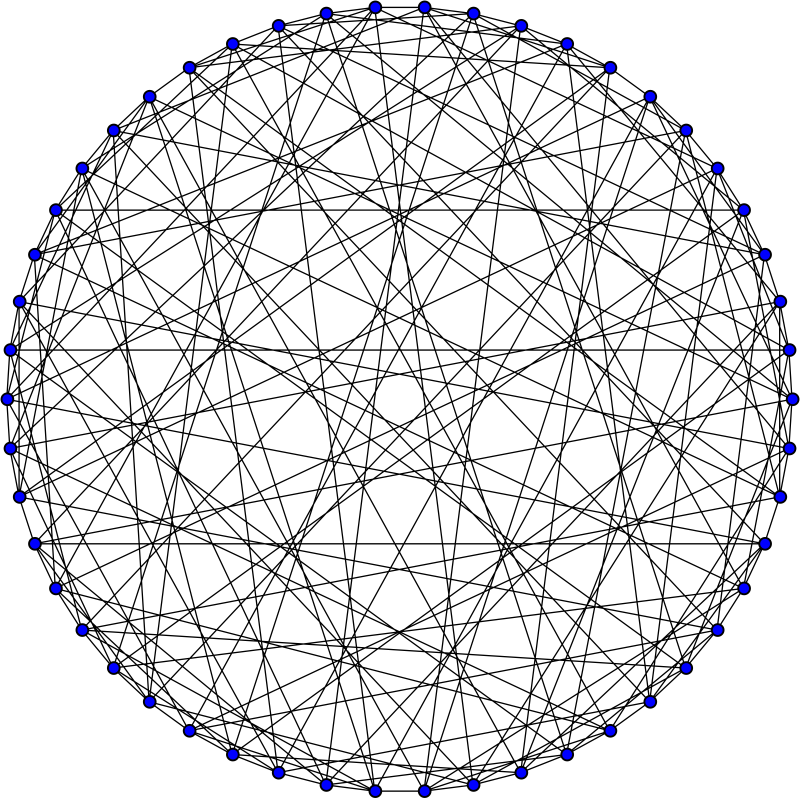
\includegraphics[scale=0.7]{img/Hoffman-Singleton_graph.png}%
        }
     \end{column}
  \end{columns}
\end{frame}   

\subsection{Fortemente Regular}

\begin{frame}
\frametitle{Nº Envoltório}
\framesubtitle{diâmetro 2 - Fortemente Regular}
  \begin{columns}[T]
    \begin{column}{.4\textwidth}
     Fortemente regular $(n,k,b,c)$:
     \begin{itemize}
         \item $n$ vértices
         \item $k$-regular
         \item $b$ vizinhos em comum todo par adjacente de vértices \item $c$ vizinhos em comum todo par não adjacente de vértices
     \end{itemize}
    \end{column}
    \begin{column}{.6\textwidth}
        \centering
        \includegraphics[scale=0.6]{img/sr.png}
    \end{column}
  \end{columns}
\end{frame}

\begin{frame}
\frametitle{Nº Envoltório}
\framesubtitle{diâmetro 2 - Fortemente Regular}

\begin{theo}
Seja $G$ um grafo fortemente regular $(n,k,b,c)$ com $c=0$ então $h(G)\le 2\omega(G)$.
\end{theo}

\begin{itemize}
    \item Se $c=0$ temos $G$ composto de componentes completas.
    \item $h(K_n)=2$ 
    \item Se $G$ é desconexo $h(G)=h(C_0)+..+h(C_n)$
\end{itemize}
\end{frame}

\begin{frame}
\frametitle{Nº Envoltório}
\framesubtitle{diâmetro 2 - Fortemente Regular e $c=0$}
\centering
\begin{tikzpicture}[scale=0.7]
\node[circle,draw,fill] (v9) at (-19.5,-1) {};
\node[circle,draw,fill] (v5) at (-16.5,-1) {};
\node[circle,draw,fill] (v8) at (-19,-2) {};
\node[circle,draw,fill] (v6) at (-17,-2) {};
\node[circle,draw,fill] (v4) at (-17,0) {};
\node[circle,draw,fill] (v2) at (-19,0) {};
\node[circle,draw,fill] (v39) at (-15,-1) {};
\node[circle,draw,fill] (v35) at (-12,-1) {};
\node[circle,draw,fill] (v38) at (-14.5,-2) {};
\node[circle,draw,fill] (v36) at (-12.5,-2) {};
\node[circle,draw,fill] (v34) at (-12.5,0) {};
\node[circle,draw,fill] (v32) at (-14.5,0) {};
\node[circle,draw,fill=black!50] (v29) at (-10.5,-1) {};
\node[circle,draw,fill=black!50] (v25) at (-7.5,-1) {};
\node[circle,draw,fill] (v28) at (-10,-2) {};
\node[circle,draw,fill] (v26) at (-8,-2) {};
\node[circle,draw,fill] (v24) at (-8,0) {};
\node[circle,draw,fill] (v22) at (-10,0) {};
\draw  (v28) edge (v22);
\draw  (v22) edge (v25);
\draw  (v28) edge (v25);
\draw  (v29) edge (v26);
\draw  (v26) edge (v24);
\draw  (v29) edge (v24);
\draw  (v35) edge (v39);
\draw  (v36) edge (v32);
\draw  (v34) edge (v38);

\node[circle,draw,fill] (v29) at (-6,-1) {};
\node[circle,draw,fill=black!50] (v25) at (-3,-1) {};
\node[circle,draw,fill=black!50] (v28) at (-5.5,-2) {};
\node[circle,draw,fill=black!50] (v26) at (-3.5,-2) {};
\node[circle,draw,fill=black!50] (v24) at (-3.5,0) {};
\node[circle,draw,fill] (v22) at (-5.5,0) {};
\draw  (v22) edge (v24);
\draw  (v22) edge (v29);
\draw  (v22) edge (v28);
\draw  (v26) edge (v22);
\draw  (v22) edge (v25);
\draw  (v29) edge (v28);
\draw  (v28) edge (v26);
\draw  (v26) edge (v25);
\draw  (v25) edge (v24);
\draw  (v24) edge (v28);
\draw  (v24) edge (v26);
\draw  (v29) edge (v25);
\draw  (v25) edge (v28);
\draw  (v26) edge (v29);
\draw  (v24) edge (v29);

\node at (-18,-3.5) {$G_1(6,0,0,0)$};
\node at (-13.5,-3.5) {$G_2(6,1,0,0)$};
\node at (-9,-3.5) {$G_3(6,2,1,0)$};
\node at (-4.5,-3.5) {$G_4(6,5,4,0)$};
\end{tikzpicture}
\end{frame}

\begin{frame}
\frametitle{Nº Envoltório}
\framesubtitle{diâmetro 2 - Fortemente Regular}
\begin{theo}
Seja $G$ um grafo fortemente regular $(n,k,b,c)$ com $c>0$ então existe um $S'$ tal que $|S'| = \big\lceil \frac{k}{1+b} \big\rceil$ e $H(S')$ é um conjunto dominante.
\label{dom-gfr} 
\end{theo}
\begin{itemize}
    \item Se $c > 0$ temos $G$ diâmetro 2
    \item Dado $v$ podemos compor um $S^\prime \subseteq N(v)$
    \item A cada iteração um novo vértice em $S^\prime$ e $b+1$ em $H(S^\prime)$
    \item $N(v) \subseteq H(S^\prime)$ então $H(S^\prime)$ é dominante
\end{itemize}
\end{frame}

\begin{frame}
\frametitle{Nº Envoltório}
\framesubtitle{diâmetro 2 - Fortemente Regular e $c>0$}
\begin{tikzpicture}
\node[circle,draw,fill=black!50,label=left:$v$] (v1) at (-13.5,-1) {};
\node[circle,draw,fill] (v3) at (-13.5,0.5) {};
\node[circle,draw,fill] (v9) at (-15,-1) {};
\node[circle,draw,fill] (v7) at (-13.5,-2.5) {};
\node[circle,draw,fill] (v5) at (-12,-1) {};
\node[circle,draw,fill] (v8) at (-14.5,-2) {};
\node[circle,draw,fill] (v6) at (-12.5,-2) {};
\node[circle,draw,fill] (v4) at (-12.5,0) {};
\node[circle,draw,fill] (v2) at (-14.5,0) {};
\draw  (v1) edge (v2);
\draw  (v1) edge (v3);
\draw  (v1) edge (v4);
\draw  (v1) edge (v5);
\draw  (v1) edge (v6);
\draw  (v7) edge (v1);
\draw  (v1) edge (v8);
\draw  (v1) edge (v9);

\node[circle,draw,fill=black!50,label=left:$v$] (v31) at (-9,-1) {};
\node[circle,draw,fill] (v33) at (-9,0.5) {};
\node[circle,draw,fill] (v39) at (-10.5,-1) {};
\node[circle,draw,fill] (v37) at (-9,-2.5) {};
\node[circle,draw,fill] (v35) at (-7.5,-1) {};
\node[circle,draw,fill=black!50] (v38) at (-10,-2) {};
\node[circle,draw,fill=black!50] (v36) at (-8,-2) {};
\node[circle,draw,fill=black!50] (v34) at (-8,0) {};
\node[circle,draw,fill=black!50] (v32) at (-10,0) {};
\draw  (v31) edge (v32);
\draw  (v31) edge (v33);
\draw  (v31) edge (v34);
\draw  (v31) edge (v35);
\draw  (v31) edge (v36);
\draw  (v37) edge (v31);
\draw  (v31) edge (v38);
\draw  (v31) edge (v39);

\node[circle,draw,fill=black!50,label=left:$v$] (v21) at (-4.5,-1) {};
\node[circle,draw,fill] (v23) at (-4.5,0.5) {};
\node[circle,draw,fill] (v27) at (-4.5,-2.5) {};
\node[circle,draw,fill=black!50] (v28) at (-5.5,-2) {};
\node[circle,draw,fill=black!50] (v26) at (-3.5,-2) {};
\node[circle,draw,fill=black!50] (v24) at (-3.5,0) {};
\node[circle,draw,fill=black!50] (v22) at (-5.5,0) {};
\draw  (v34) edge (v33);
\draw  (v36) edge (v35);
\draw  (v37) edge (v38);
\draw  (v39) edge (v32);

\node at (-13.5,-3.5) {$N(v)|$ $G_1(n,k,0,c)$};
\node at (-9,-3.5) {$N(v)|$ $G_2(n,k,1,c)$};
\node at (-4.5,-3.5) {$N(v)|$  $G_3(n,k,2,c)$};
\draw  (v22) edge (v21);
\draw  (v21) edge (v24);
\draw  (v24) edge (v22);
\draw  (v23) edge (v21);
\draw  (v22) edge (v23);
\draw  (v23) edge (v24);
\draw  (v28) edge (v21);
\draw  (v21) edge (v26);
\draw  (v27) edge (v28);
\draw  (v27) edge (v26);
\draw  (v21) edge (v27);
\draw  (v26) edge (v28);
\end{tikzpicture}
\end{frame}



\begin{frame}
\frametitle{Nº Envoltório}
\framesubtitle{diâmetro 2 - Fortemente Regular}
\begin{lem}
Considere a i-ésima iteração do algoritmo em um grafo $G$ fortemente regular $(n,k,b,c)$ com $c>0$. Se $O_i \neq \emptyset$, então $|H(S_i)|\geq (c+1) \times |H(S_{i-1})|+1$.
\label{pior-caso-hs-sr}
\end{lem}
\begin{proposition} 
No máximo haverá $i=\big \lceil \log_{c+1}(kc+1) \big \rceil$ iterações.
\end{proposition}
\begin{theo}
Seja $G$ um grafo fortemente regular e $c>0$ então $h(G) \le \big \lceil \log_{c+1}(kc+1) \big \rceil + 1$.
\end{theo}
\end{frame}



\begin{frame}
\frametitle{Nº Envoltório}
%\framesubtitle{diâmetro 2 - exemplos}
\centering
%\tiny
\resizebox{.9\textwidth}{!}{%
%\small
\begin{tabular}{r|c|c|c|c|c}
& & \multicolumn{2}{c|}{\textbf{Diâmetro 2}} 
& \multicolumn{2}{c}{\textbf{Fortemente Regular}} \\ 
\textbf{Grafo} & \textbf{h} & \textbf{Corol. 3.4}
& \textbf{Corol. 3.13} & \textbf{Corol. 3.22} & \textbf{Teor. 3.25}  \\ \hline
$C_5$ (5,2,0,1) & 3  & 3 & 3 & 3 & 3 \\ \hline
Petersen (10,3,0,1) & 3  & 4 & 3 & 4 & 3\\ \hline
Clebsch (16,5,0,2)  & 3 & 6 & 4 & 6 & 3 \\ \hline
(4,4)-Hook (16,6,2,2) & 2  & 7 & 4 & 3 & 3\\ \hline
Hoffman-Singleton (50,7,0,1) & 4 & 8 & 4 & 8 & 4 \\ \hline
Gewirtz (56,10,0,2) & 3  & 11 & 4 & 11 & 4\\ \hline
Brouwer-Haemers (81,20,1,6) & 2 & 21 & 5 & 11 & 3\\ \hline
$M_{22}$ (77,16,0,4) & 2  & 17 & 5 & 17 & 4\\ \hline
$H(2,10)$ (100,18,8,2) & 2 & 19 & 5 & 3 & 4\\ \hline
Higman-Sims (100,22,0,6) & 2  & 23 & 6 & 23 & 4\\ \hline
$1^{st}$ sub. of McLaughlin (112,30,2,10) & 2 & 113 & 8 & 5 & 3\\ \hline
Cameron (231,30,9,3) & 2  & 31 & 6 & 4 & 4 \\ \hline
Berlekamp-van L. (243,22,1,2) & 3 & 23 & 6 & 12 & 4 \\ \hline
McLaughlin (275,112,30,56)  & 2   & 113 & 8 & 5 & 3\\ \hline
Grassmann $J_2(6,2)$ (651,90,33,9) & 2 & 91 & 8 & 4 & 4 \\ \hline
G2(4) (416,100,36,20) & 2 & 101 & 8 & 4  & 3  \\ \hline
Games (729,112,1,20) & * &  113 & 8 & 57 & 4 \\ %\hline
\end{tabular}%
}
\end{frame}

\begin{frame}
\centering
\textbf{Resultados para Nº Carathéodory}
\end{frame}

\section{Resultados Carathéodory}
\begin{frame}
\frametitle{Nº Carathéodory}
\framesubtitle{diâmetro 2}
\begin{columns}[T]
 \begin{column}{.5\textwidth}
\begin{proposition}
Considere $G$ um grafo de diâmetro 2 com vértice de corte, então $c(G) = 2$.
\end{proposition}
\begin{itemize}
    \item Um conjunto Carathéodory $S$ com $S\ge 3$ o vértice de corte não pode ser o parcial
    \item Os vértices de $S$ estão em componentes distintas
    \item O parcial está em componentes distintas de outros vértices de $S$ e não pode ser o vértice de corte
    \item O parcial não existe
\end{itemize}
\end{column}
\begin{column}{.5\textwidth}
\centering
\begin{tikzpicture}[scale=0.5]
\node[circle,draw,fill=black!50] (v1) at (-13.5,-1) {};
\node[circle,draw,fill] (v3) at (-13.5,0.5) {};
\node[circle,draw,fill] (v9) at (-15,-1) {};
\node[circle,draw] (v7) at (-13.5,-2.5) {};
\node[circle,draw] (v5) at (-12,-1) {};
\node[circle,draw] (v8) at (-14.5,-2) {};
\node[circle,draw] (v6) at (-12.5,-2) {};
\node[circle,draw] (v4) at (-12.5,0) {};
\node[circle,draw] (v2) at (-14.5,0) {};
\draw  (v1) edge (v2);
\draw  (v1) edge (v3);
\draw  (v1) edge (v4);
\draw  (v1) edge (v5);
\draw  (v1) edge (v6);
\draw  (v7) edge (v1);
\draw  (v1) edge (v8);
\draw  (v1) edge (v9);

\node[circle,draw,fill=black!50] (v31) at (-9,-1) {};
\node[circle,draw,fill] (v33) at (-9,0.5) {};
\node[circle,draw,fill] (v39) at (-10.5,-1) {};
\node[circle,draw] (v37) at (-9,-2.5) {};
\node[circle,draw] (v35) at (-7.5,-1) {};
\node[circle,draw] (v38) at (-10,-2) {};
\node[circle,draw] (v36) at (-8,-2) {};
\node[circle,draw,fill=black!50] (v34) at (-8,0) {};
\node[circle,draw,fill=black!50] (v32) at (-10,0) {};
\draw  (v31) edge (v32);
\draw  (v31) edge (v33);
\draw  (v31) edge (v34);
\draw  (v31) edge (v35);
\draw  (v31) edge (v36);
\draw  (v37) edge (v31);
\draw  (v31) edge (v38);
\draw  (v31) edge (v39);

\node[circle,draw,fill=black!50] (v21) at (-4.5,-1) {};
\node[circle,draw,fill] (v23) at (-4.5,0.5) {};
\node[circle,draw,fill=black!50] (v29) at (-6,-1) {};
\node[circle,draw,fill=black!50] (v27) at (-4.5,-2.5) {};
\node[circle,draw,fill=black!50] (v25) at (-3,-1) {};
\node[circle,draw,fill=black!50] (v28) at (-5.5,-2) {};
\node[circle,draw,fill=black!50] (v26) at (-3.5,-2) {};
\node[circle,draw,fill] (v24) at (-3.5,0) {};
\node[circle,draw,fill=black!50] (v22) at (-5.5,0) {};
\draw  (v21) edge (v22);
\draw  (v21) edge (v23);
\draw  (v21) edge (v24);
\draw  (v21) edge (v25);
\draw  (v21) edge (v26);
\draw  (v27) edge (v21);
\draw  (v21) edge (v28);
\draw  (v21) edge (v29);
\draw  (v24) edge (v25);
\draw  (v26) edge (v25);
\draw  (v28) edge (v29);
\draw  (v28) edge (v27);
\draw  (v22) edge (v29);
\draw  (v23) edge (v22);

\draw  (v34) edge (v33);
\draw  (v36) edge (v35);
\draw  (v37) edge (v38);
\draw  (v39) edge (v32);
\end{tikzpicture}
\end{column}
\end{columns}
\end{frame}

\begin{frame}
\frametitle{Nº Carathéodory}
\framesubtitle{diâmetro 2}
\begin{columns}[T]
\begin{column}{.4\textwidth}
\begin{coro}
    Seja $G$ um grafo MST $C_5[p,q,r,s,t]$ e $|p|$, $|q|$, $|r|$, $|s|$ e $|t|$ for maior que 1 então $c(G) = 2$.
\end{coro}
\begin{itemize}
    \item Um conjunto Carathéodory $S$ com $S\ge 3$ contem 2 ou mais vértices não adjacentes
    \item Qualquer 2 vértices não adjacentes são um conjunto envoltório
    \item $\not \exists S^\prime \subset S$ tal que $S^\prime$ é envoltório
\end{itemize}
\end{column}
\begin{column}{.6\textwidth}
\begin{tikzpicture}
\node[draw,circle,label=$s_0$,fill] (v4) at (-1,-4) {};
\node[circle,draw,label=right:$t_0$,fill=black!70] (v5) at (-3,-3) {};
\node[circle,draw,label=below:$p_0$,fill] (v1) at (-2,-1) {};
\node[circle,draw,label=below:$q_0$,fill] (v2) at (0,-1) {};
\node[draw,circle,label=left:$r_0$,fill=black!70] (v3) at (1,-3) {};
\draw (v1) -- (v2) -- (v3) -- (v4) -- (v5) -- (v1);
\node[draw,circle,label=$p_1$,fill=black!50] (v6) at (-2.5,-0.5) {};
\node[draw,circle,label=$q_1$,fill=black!50] (v9) at (0.5,-0.5) {};
\node[draw,circle,label=$s_1$,fill=black!50] (v13) at (-1,-5) {};
\node[draw,circle,label=$s_2$,fill=black!50] (v12) at (-1,-6) {};
\node[draw,circle,label=right:$r_1$,fill=black!50] (v15) at (2,-3) {};
\node[draw,circle,label=right:$r_2$,fill=black!50] (v14) at (3,-3) {};
\node[draw,circle,label=left:$t_1$,fill=black!50] (v8) at (-4,-3) {};
\node[draw,circle,label=left:$t_2$,fill=black!50] (v7) at (-5,-3) {};
	
\draw  (v6) edge (v7);
\draw  (v6) edge (v8);
\draw  (v6) edge (v5);
\draw  (v6) edge (v9);
\draw  (v6) edge (v2);
\draw  (v12) edge (v7);
\draw  (v13) edge (v7);
\draw  (v8) edge (v4);
\draw  (v4) edge (v7);
\draw  (v8) edge (v13);
\draw  (v8) edge (v12);
\draw  (v14) edge (v12);
\draw  (v14) edge (v13);
\draw  (v14) edge (v4);
\draw  (v15) edge (v4);
\draw  (v13) edge (v15);
\draw  (v12) edge (v15);
\draw  (v9) edge (v3);
\draw  (v9) edge (v15);
\draw  (v14) edge (v9);
\draw  (v1) edge (v9);
\draw  (v1) edge (v7);
\draw  (v1) edge (v2);
\draw  (v14) edge (v2);
\draw  (v1) edge (v8);
\draw  (v2) edge (v15);
\draw  (v3) edge (v13);
\draw  (v13) edge (v5);
\draw  (v3) edge (v12);
\draw  (v12) edge (v5);
\end{tikzpicture}
\end{column}
\end{columns}
\end{frame}


\begin{frame}
\frametitle{Implementações}
\centering
\textbf{Implementações e Outras Contribuições}
\end{frame}

\section{Implementações}
\subsection{Moore}
\begin{frame}
\frametitle{Implementações}
\framesubtitle{Grafos de Moore}
Um Grafo de {\it Moore} é um Grafo regular de grau $d$ e distância $k$ tal que o número de vértices é igual ao limitante superior: $$1 + d\sum_{i=0}{k-1}(d-1)^i$$
\end{frame}


\begin{frame}
\frametitle{Implementações}
\framesubtitle{Grafos de Moore}
\begin{itemize}
    \item{Diâmetro 2, só são possíveis para os valores de $k$ igual a 2, 3, 7 ou 57 [Hoffman e Singleton, 1960]}
    \item{Não existem grafos de Moore com $\Delta \geq 3$ e $d\geq 3$, ou seja eles possuem diâmetro no máximo 2 [Bannai, 1973]}
\end{itemize}
\end{frame}

\begin{frame}
\frametitle{Implementações}
\framesubtitle{Grafo de Moore - $k={2,3,7}$}
Grafos de Moore conhecidos:
\begin{itemize}
    \item{$k=2$ Ciclo de tamanho 5}
    \item{$k=3$ Petersen}
    \item{$k=7$ Hoffman-Singleton}
\end{itemize}
\end{frame}

\begin{frame}
\frametitle{Implementações}
\framesubtitle{Grafo de Moore 57-regular - Sabemos}
\begin{itemize}
    \item{Sua existência permanece em aberto desde 1960}
    \item{57 regular, 3250 vértices, 92625 arestas, diâmetro 2 e cintura 5}
    \item{Não é distância-transitivo [Aschbacher, 1971]}
    \item{Não é vértice-transitivo [Cameron, 1983]}
    \item{Possui ao menos 375 automorfismo [Macaj, 2010]}
\end{itemize}
\end{frame}



\begin{frame}
\frametitle{Implementações}
\framesubtitle{Algoritmo - Grafos de Moore - Construção esqueleto}
\begin{figure}[h]
\centering
\begin{tikzpicture}[scale=0.8]
\node[circle,draw,label=above:$v_{k^2-2}$] (v2) at (5,0) {};
\node[circle,draw,label=above:$v_{k^2}$] (v1) at (0,0) {};
\node[circle,draw,label=above:$v_{k^2-1}$] (v3) at (-5,0) {};
\draw  (v1) edge (v2);
\draw  (v1) edge (v3);
\end{tikzpicture}
\label{fig-execucao-moore}
\end{figure}
\end{frame}

\begin{frame}
\frametitle{Implementações}
\framesubtitle{Algoritmo - Grafos de Moore - Construção esqueleto}
%\begin{turn}{-90}
\begin{figure}[h]
\centering
\begin{tikzpicture}[scale=0.8]
\node[circle,draw,label=above:$v_{k^2-2}$,fill] (v2) at (5,0) {};
\node[circle,draw,label=below:$v_{0}$] (v4) at (4,-3.5) {};
\node[circle,draw,label=above:$v_{k^2}$] (v1) at (0,0) {};
\node[circle,draw,label=above:$v_{k^2-1}$,fill] (v3) at (-5,0) {};
\node[circle,draw,label=below:$v_{k-1}$] (v7) at (-4,-3.5) {};
\node[circle,draw,label=below:$v_{1}$] (v5) at (5,-5) {};
\node[circle,draw,label=below:$v_{k-2}$] (v6) at (6,-6.5) {};
\node[circle,draw,label=below:$v_{k}$] (v8) at (-5,-5) {};
\node[circle,draw,label=below:$v_{2k-3}$] (v9) at (-6,-6.5) {};
\draw  (v1) edge (v2);
\draw  (v1) edge (v3);
\draw  (v2) edge (v4);
\draw  (v2) edge (v5);
\draw  (v2) edge (v6);
\draw  (v3) edge (v7);
\draw  (v3) edge (v8);
\draw  (v3) edge (v9);
\draw[dotted]  (v5) edge (v6);
\draw[dotted]  (v8) edge (v9);
\end{tikzpicture}
\label{fig-execucao-moore}
\end{figure}
%\end{turn}
\end{frame}

\begin{frame}
\frametitle{Implementações}
\framesubtitle{Algoritmo - Grafos de Moore - Construção esqueleto}
%\begin{turn}{-90}
\begin{figure}[h]
\centering
\begin{tikzpicture}[scale=0.8]
\node[circle,draw,label=above:$v_{k^2-2}$,fill] (v2) at (5,0) {};
\node[circle,draw,label=below:$v_{0}$] (v4) at (4,-3.5) {};
\node[circle,draw,label=above:$v_{k^2}$] (v1) at (0,0) {};
\node[circle,draw,label=above:$v_{k^2-1}$,fill] (v3) at (-5,0) {};
\node[circle,draw,label=below:$v_{k-1}$] (v7) at (-4,-3.5) {};
\node[circle,draw,label=below:$v_{1}$] (v5) at (5,-5) {};
\node[circle,draw,label=below:$v_{k-2}$] (v6) at (6,-6.5) {};
\node[circle,draw,label=below:$v_{k}$] (v8) at (-5,-5) {};
\node[circle,draw,label=below:$v_{2k-3}$] (v9) at (-6,-6.5) {};
\draw  (v1) edge (v2);
\draw  (v1) edge (v3);
\draw  (v2) edge (v4);
\draw  (v2) edge (v5);
\draw  (v2) edge (v6);
\draw  (v3) edge (v7);
\draw  (v3) edge (v8);
\draw  (v3) edge (v9);
\draw  (v4) edge (v7);
\draw  (v5) edge (v8);
\draw  (v6) edge (v9);
\draw[dotted]  (v5) edge (v6);
\draw[dotted]  (v8) edge (v9);
\end{tikzpicture}
\label{fig-execucao-moore}
\end{figure}
%\end{turn}
\end{frame}



\begin{frame}
\frametitle{Implementações}
\framesubtitle{Algoritmo - Grafos de Moore - Construção esqueleto}
%\begin{turn}{-90}
\begin{figure}[h]
\centering
\begin{tikzpicture}[scale=0.8]
\node[circle,draw,label=above:$v_{k^2-2}$,fill] (v2) at (5,0) {};
\node[circle,draw,label=below:$v_{0}$] (v4) at (4,-3.5) {};
\node[circle,draw,label=above:$v_{k^2}$] (v1) at (0,0) {};
\node[circle,draw,label=above:$v_{k^2-1}$,fill] (v3) at (-5,0) {};
\node[circle,draw,label=below:$v_{k-1}$] (v7) at (-4,-3.5) {};
\node[circle,draw,label=below:$v_{1}$] (v5) at (5,-5) {};
\node[circle,draw,label=below:$v_{k-2}$] (v6) at (6,-6.5) {};
\node[circle,draw,label=below:$v_{k}$] (v8) at (-5,-5) {};
\node[circle,draw,label=below:$v_{2k-3}$] (v9) at (-6,-6.5) {};
\draw  (v1) edge (v2);
\draw  (v1) edge (v3);
\draw  (v2) edge (v4);
\draw  (v2) edge (v5);
\draw  (v2) edge (v6);
\draw  (v3) edge (v7);
\draw  (v3) edge (v8);
\draw  (v3) edge (v9);
\draw  (v4) edge (v7);
\draw  (v5) edge (v8);
\draw  (v6) edge (v9);
\draw[dashed] (v4) edge[red] (v8);
\draw[dashed]  (v5) edge[red] (v7);
\draw[dashed]  (v6) edge[red] (v7);
\draw[dashed]  (v4) edge[red] (v9);
\draw[dashed]  (v5) edge[red] (v9);
\draw[dashed]  (v6) edge[red] (v8);
\draw[dotted]  (v5) edge (v6);
\draw[dotted]  (v8) edge (v9);
\end{tikzpicture}
\label{fig-execucao-moore}
\end{figure}
%\end{turn}
\end{frame}


\begin{frame}
\frametitle{Implementações}
\framesubtitle{Algoritmo - Grafos de Moore - Construção esqueleto}
\centering
\begin{turn}{-90}
\begin{tikzpicture}
\node[circle,draw,label=$v_{k^2-2}$,fill] (v2) at (-2.5,4) {};
\node[circle,draw,label=$v_{0}$,fill] (v4) at (-1,3) {};
\node[circle,draw,label=left:$v_{k^2}$] (v1) at (-2.5,0.5) {};
\node[circle,draw,label=below:$v_{k^2-1}$,fill] (v3) at (-2.5,-3.5) {};
\node[circle,draw,label=below:$v_{k-1}$,fill] (v7) at (-1,-2.5) {};
\node[circle,draw,label=$v_{k-3}$,fill] (v5) at (1,4) {};
\node[circle,draw,label=$v_{k-2}$,fill] (v6) at (2.3,5.5) {};
\node[circle,draw,label=below:$v_{2k-4}$,fill] (v8) at (1,-3.5) {};
\node[circle,draw,label=below:$v_{2k-3}$,fill] (v9) at (2.4,-4.8) {};
\draw  (v1) edge (v2);
\draw  (v1) edge (v3);
\draw  (v2) edge (v4);
\draw  (v2) edge (v5);
\draw  (v2) edge (v6);
\draw  (v3) edge (v7);
\draw  (v3) edge (v8);
\draw  (v3) edge (v9);
\draw  (v4) edge (v7);
\draw  (v5) edge (v8);
\draw  (v6) edge (v9);
\draw[dotted]  (v5) edge (v4);
\draw[dotted]  (v8) edge (v7);
\node[draw,circle,label=left:$v_{2k-2}$] (v10) at (-0.5,2) {};
\node[draw,circle,label=left:$v_{2k-1}$] (v11) at (-0.5,-1) {};
\node[draw,circle] (v12) at (0.5,2) {};
\node[draw,circle] (v13) at (0.5,-1) {};
\node[draw,circle,label=right:$v_{k^2-k-1}$] (v15) at (1.5,-1) {};
\node[draw,circle,label=right:$v_{k^2-k-2}$] (v14) at (1.5,2) {};
\draw  (v4) edge (v10);
\draw  (v10) edge (v8);
\draw  (v7) edge (v11);
\draw  (v11) edge (v5);
\draw  (v4) edge (v12);
\draw  (v9) edge (v12);
\draw  (v7) edge (v13);
\draw  (v13) edge (v6);
\draw  (v5) edge (v14);
\draw  (v14) edge (v9);
\draw  (v8) edge (v15);
\draw  (v15) edge (v6);

\draw[dotted]  (v10) edge (v12);
\draw[dotted]  (v13) edge (v11);
\draw[dotted]  (v12) edge (v14);
\draw[dotted]  (v15) edge (v13);
\end{tikzpicture}
\end{turn}
\end{frame}


\begin{frame}
\frametitle{Implementações}
\framesubtitle{Algoritmo - Grafos de Moore - Esqueleto}
\centering
\begin{turn}{-90}
\begin{tikzpicture}
\node[circle,draw,label=$v_{k^2-2}$,fill] (v2) at (-2.5,4) {};
\node[circle,draw,label=$v_{0}$,fill] (v4) at (-1,3) {};
\node[circle,draw,label=left:$v_{k^2}$,fill] (v1) at (-2.5,0.5) {};
\node[circle,draw,label=below:$v_{k^2-1}$,fill] (v3) at (-2.5,-3.5) {};
\node[circle,draw,label=below:$v_{k-1}$,fill] (v7) at (-1,-2.5) {};
\node[circle,draw,label=$v_{k-3}$,fill] (v5) at (1,4) {};
\node[circle,draw,label=$v_{k-2}$,fill] (v6) at (2.3,5.5) {};
\node[circle,draw,label=below:$v_{2k-4}$,fill] (v8) at (1,-3.5) {};
\node[circle,draw,label=below:$v_{2k-3}$,fill] (v9) at (2.4,-4.8) {};

\draw  (v1) edge (v2);
\draw  (v1) edge (v3);
\draw  (v2) edge (v4);
\draw  (v2) edge (v5);
\draw  (v2) edge (v6);
\draw  (v3) edge (v7);
\draw  (v3) edge (v8);
\draw  (v3) edge (v9);
\draw  (v4) edge (v7);
\draw  (v5) edge (v8);
\draw  (v6) edge (v9);
\draw[dotted]  (v5) edge (v4);
\draw[dotted]  (v8) edge (v7);
\node[circle,draw,label=$v_{k^2-k}$] (v16) at (-2,2.5) {};
\node[circle,draw,label=below:$v_{k^2-3}$] (v17) at (-2,-2) {};
\draw  (v1) edge (v16);
\draw  (v1) edge (v17);

\node[draw,circle,label=left:$v_{2k-2}$] (v10) at (-0.5,2) {};
\node[draw,circle,label=left:$v_{2k-1}$] (v11) at (-0.5,-1) {};
\node[draw,circle] (v12) at (0.5,2) {};
\node[draw,circle] (v13) at (0.5,-1) {};
\node[draw,circle,label=right:$v_{k^2-k-1}$] (v15) at (1.5,-1) {};
\node[draw,circle,label=right:$v_{k^2-k-2}$] (v14) at (1.5,2) {};

\draw  (v4) edge (v10);
\draw  (v10) edge (v8);
\draw  (v7) edge (v11);
\draw  (v11) edge (v5);
\draw  (v4) edge (v12);
\draw  (v9) edge (v12);
\draw  (v7) edge (v13);
\draw  (v13) edge (v6);
\draw  (v5) edge (v14);
\draw  (v14) edge (v9);
\draw  (v8) edge (v15);
\draw  (v15) edge (v6);

\draw[dotted]  (v10) edge (v12);
\draw[dotted]  (v13) edge (v11);
\draw[dotted]  (v12) edge (v14);
\draw[dotted]  (v15) edge (v13);
\draw[dotted]  (v16) edge (v17);
\end{tikzpicture}
\end{turn}
\end{frame}



\begin{frame}
\frametitle{Implementações}
\framesubtitle{Algoritmo - Grafos de Moore - Complemento com Combinações}
\centering
\begin{turn}{-90}
\begin{tikzpicture}
\node[circle,draw,fill] (v2) at (-2.5,4) {};
\node[circle,draw,fill] (v4) at (-1,3) {};
\node[circle,draw,fill] (v1) at (-2.5,0.5) {};
\node[circle,draw,fill] (v3) at (-2.5,-3.5) {};
\node[circle,draw,fill] (v7) at (-1,-2.5) {};
\node[circle,draw,fill] (v5) at (1,4) {};
\node[circle,draw,fill] (v6) at (2.3,5.5) {};
\node[circle,draw,fill] (v8) at (1,-3.5) {};
\node[circle,draw,fill] (v9) at (2.4,-4.8) {};

\draw  (v1) edge (v2);
\draw  (v1) edge (v3);
\draw  (v2) edge (v4);
\draw  (v2) edge (v5);
\draw  (v2) edge (v6);
\draw  (v3) edge (v7);
\draw  (v3) edge (v8);
\draw  (v3) edge (v9);
\draw  (v4) edge (v7);
\draw  (v5) edge (v8);
\draw  (v6) edge (v9);
\draw[dotted]  (v5) edge (v4);
\draw[dotted]  (v8) edge (v7);
\node[circle,draw] (v16) at (-1.5,1.5) {};
\node[circle,draw] (v17) at (-1.5,-0.5) {};
\draw  (v1) edge (v16);
\draw  (v1) edge (v17);

\node[draw,circle] (v10) at (-0.5,2) {};
\node[draw,circle] (v11) at (-0.5,-1) {};
\node[draw,circle] (v12) at (0.5,1.5) {};
\node[draw,circle] (v13) at (0.5,-0.5) {};
\node[draw,circle] (v15) at (1.5,-1) {};
\node[draw,circle] (v14) at (1.5,2) {};

\draw  (v4) edge (v10);
\draw  (v10) edge (v8);
\draw  (v7) edge (v11);
\draw  (v11) edge (v5);
\draw  (v4) edge (v12);
\draw  (v9) edge (v12);
\draw  (v7) edge (v13);
\draw  (v13) edge (v6);
\draw  (v5) edge (v14);
\draw  (v14) edge (v9);
\draw  (v8) edge (v15);
\draw  (v15) edge (v6);

\draw[dotted]  (v10) edge (v12);
\draw[dotted]  (v13) edge (v11);
\draw[dotted]  (v12) edge (v14);
\draw[dotted]  (v15) edge (v13);
\draw[dotted]  (v16) edge (v17);

\draw[dashed]  (v16) edge[red] (v10);
\draw[dashed]  (v16) edge[red] (v12);
\draw[dashed]  (v16) edge[red] (v14);
\draw[dashed]  (v13) edge[red] (v16);
\draw[dashed]  (v15) edge[red] (v16);
\draw[dashed]  (v16) edge[red] (v11);
\draw[dashed]  (v17) edge[red] (v10);
\draw[dashed]  (v12) edge[red] (v17);
\draw[dashed]  (v13) edge[red] (v17);
\draw[dashed]  (v17) edge[red] (v15);
\draw[dashed]  (v17) edge[red] (v14);
\draw[dashed]  (v13) edge[red] (v10);
\draw[dashed]  (v10) edge[red] (v15);
\draw[dashed]  (v11) edge[red] (v12);
\draw[dashed]  (v12) edge[red] (v11);
\draw[dashed]  (v12) edge[red] (v15);
\draw[dashed]  (v14) edge[red] (v13);
\draw[dashed]  (v11) edge[red] (v14);
\draw[dashed]  (v10) edge[red] (v14);
\draw[dashed] (v11) edge[red] (v15);
\draw[dashed]  (v12) edge[red] (v14);
\draw[dashed]  (v13) edge[red] (v15);
\end{tikzpicture}
\end{turn}
\end{frame}


\subsection{Convexidade}
\begin{frame}
\frametitle{Implementações}
\framesubtitle{Algoritmos - Convexidade $P_3$}
\centering
\adjustbox{max width=\textwidth}{
    \begin{tabular}{l|l|l}
               & \textbf{Algoritmo}         & \textbf{Abordagem}  \\ \hline
    \multicolumn{1}{l|}{1} & NumeroEnvoltorio(G(V,E))   & Exponencial         \\ \hline
    \multicolumn{1}{l|}{2} & NumeroCaratheodory(G(V,E)) & Exponencial         \\ \hline
    \multicolumn{1}{l|}{3} & AproxNEnvoltoria(G(V,E))   & Aproximativo Guloso \\ \hline
    \multicolumn{1}{l|}{4} & AproxNCaratheodory(G(V,E)) & Aproximativo Guloso \\ %\hline
    \end{tabular}
}
\end{frame}


\begin{frame}
\frametitle{Implementações}
\framesubtitle{Definição}
  \begin{columns}[T]
    \begin{column}{.3\textwidth}
    \begin{algorithm}[H]
        \SetAlFnt{\tiny}
        \SetAlCapFnt{\small}
        \SetAlCapNameFnt{\small}
        \SetAlgoLined
        \DontPrintSemicolon
        \LinesNumbered
        \SetAlgoLined
        \BlankLine
        \Entrada{$G(V,E)$ e $S | S \subseteq V(G)$}
        \Saida{$S^\prime$, menor conjunto convexo contendo S}
        \BlankLine

        $fila \gets S$ \\
        $S^\prime \gets \emptyset$ \\
        $cont[1...|V|] \gets 0$\\
        \Enqto{$fila \ne \emptyset$}{
            $v \gets remover(fila)$\\
            $cont[v] \gets 2$\\
            $S^\prime  \gets S^\prime \cup \{v\}$\\
            \ParaCada{$w \in Adj[v]$}{
                \Se{($cont[w] = 1)$}{
                    $inserir(w, fila)$\\
                }
                $cont[w] \gets cont[w] + 1$\\
            }
        }
        \Retorna{$S^\prime$}    
        \caption{$H(G(V,E),S)$}
    \end{algorithm}
    \end{column}
    \begin{column}{.3\textwidth}
        \begin{algorithm}[H]
        \SetAlFnt{\tiny}
        \SetAlCapFnt{\small}
        \SetAlCapNameFnt{\small}
        \SetAlgoLined
        \DontPrintSemicolon
        \LinesNumbered
        \SetAlgoLined
        \BlankLine
        \Entrada{$G(V,E)$, $S \subseteq V(G)$}
        \Saida{Verdadeiro se $S$ é um conjunto de Carathéodory}
        \BlankLine
        $S^\prime \gets H(G(V,E),S)$ \\
        \ParaCada{$u \in S$}{
            $S^{\prime \prime} \gets H(G(V,E),S \setminus \{u\})$ \\
            $S^\prime \gets S^\prime \setminus S^{\prime \prime}$ \\
        }
        \Retorna{$S^\prime \ne \emptyset$} 
        \caption{$ConjCarat(G(V,E),S)$} 
    \end{algorithm}
    \end{column}
    \begin{column}{.3\textwidth}
        \begin{algorithm}[H]
            \SetAlFnt{\tiny}
            \SetAlCapFnt{\small}
            \SetAlCapNameFnt{\small}
            \SetAlgoLined
            \DontPrintSemicolon
            \LinesNumbered
            \SetAlgoLined
            \BlankLine
            \Entrada{$G(V,E)$, $S \subseteq V(G)$}
            \Saida{Verdadeiro se $H(S) = V(G)$}
            \BlankLine
            $S^\prime \gets H(G(V,E),S)$ \\
            \Retorna{$|S^\prime| = |V|$} 
        \caption{$ConjEnv(G(V,E),S)$}   
        \end{algorithm}
    \end{column}
  \end{columns}
\end{frame}

\begin{frame}
\frametitle{Implementações}
\framesubtitle{NumeroEnvoltorio(G(V,E))}
  \begin{columns}[T]
    \begin{column}{.5\textwidth}
    \begin{algorithm}[H]
        \caption{$NumeroEnvoltorio(G(V,E))$}
        \SetAlFnt{\tiny}
        \SetAlCapFnt{\small}
        \SetAlCapNameFnt{\small}
        \SetAlgoLined
        \DontPrintSemicolon
        \LinesNumbered
        \SetAlgoLined
        \BlankLine
        \Entrada{$G(V,E)$}
        \Saida{h(G)}
        \BlankLine
        $h \gets 0$\\
        $k \gets 2$\\
        \Enqto{$k \le |V(G)| \land h = 0$}{
            \Se{$ConjuntoEnvoltoriaK(G(V,E),k)$}{
                $h \gets k$\\
            }
            $k \gets k + 1$\\          
        }
        \Retorna{h}
     \end{algorithm}
    \end{column}
    \begin{column}{.5\textwidth}
        \begin{algorithm}[H]
            \caption{$ConjuntoEnvoltoriaK(G(V,E),k)$}
            \label{alg:busca-conjunto-envoltoria-p3}
            \SetAlFnt{\tiny}
            \SetAlCapFnt{\small}
            \SetAlCapNameFnt{\small}
            \SetAlgoLined
            \DontPrintSemicolon
            \LinesNumbered
            \SetAlgoLined
            \BlankLine
            \Entrada{$G(V,E)$, inteiro $k \ge 1$}
            \Saida{Verdadeiro se $G(V,E)$ tem um conjunto envoltório de tamanho k}
            \BlankLine
            \BlankLine
            $c_{nk} \gets \frac{n!}{k!(n-k)!}$\\
            \Para{i de 1 até $c_{nk}$}{
                $S \gets Combinacao(V, k, i)$\\
                \Se{$ConjuntoEnvoltoria(G(V,E),S)$}{
                    \Retorna{\textbf{verdadeiro}}
                } 
            }
            \Retorna{\textbf{falso}} 
        \end{algorithm}
    \end{column}
  \end{columns}
\end{frame}

\begin{frame}
\frametitle{Implementações}
\framesubtitle{NumeroCaratheodory(G(V,E))}
  \begin{columns}[T]
    \begin{column}{.5\textwidth}
    \begin{algorithm}[H]
        \label{alg:numero-caratheodory-p3}
        \SetAlFnt{\tiny}
        \SetAlCapFnt{\small}
        \SetAlCapNameFnt{\small}
        \SetAlgoLined
        \DontPrintSemicolon
        \LinesNumbered
        \SetAlgoLined
        \BlankLine
        \Entrada{$G(V,E)$}
        \Saida{$c(G)$}
        \BlankLine
        $c \gets 0$\\
        $k \gets \frac{n + 1}{2}$\\
        \Enqto{$k \ge 1 \land c = 0$}{
            \Se{$ConjuntoCaratheodoryK(G(V,E),k)$}{
                $c \gets k$\\
            }
            $k \gets k - 1$\\ 
        }
        \Retorna{c}
    \caption{$NumeroCaratheodory(G(V,E))$}
    \end{algorithm}
    \end{column}
    \begin{column}{.5\textwidth}
        \begin{algorithm}[H]
            \label{alg:busca-conjunto-caratheodory-p3}
            \SetAlFnt{\tiny}
            \SetAlCapFnt{\small}
            \SetAlCapNameFnt{\small}
            \SetAlgoLined
            \DontPrintSemicolon
            \LinesNumbered
            \SetAlgoLined
            \BlankLine
            \Entrada{$G(V,E)$, inteiro $k \ge 1$}
            \Saida{Verdadeiro, se o grafo $G(V,E)$ tem um conjunto de Carathéodory de tamanho k}
            \BlankLine
            $c_{nk} \gets \frac{n!}{k!(n-k)!}$\\
            \Para{i de 1 até $c_{nk}$}{
                $S \gets Combinacao(V, k, i)$\\
                \Se{$ConjuntoCaratheodory(G(V,E),S)$}{
                    \Retorna{\textbf{verdadeiro}}
                } 
            }
            \Retorna{\textbf{falso}} 
            \caption{$ConjuntoCaratheodoryK(G(V,E),k)$}
        \end{algorithm}
    \end{column}
  \end{columns}
\end{frame}

\begin{frame}
\frametitle{Implementações}
\framesubtitle{Kernel Paralelo}
  \begin{columns}[T]
    \begin{column}{.5\textwidth}
    \begin{algorithm}[H]
        \SetAlFnt{\tiny}
        \SetAlCapFnt{\small}
        \SetAlCapNameFnt{\small}
        \SetAlgoLined
        \DontPrintSemicolon
        \LinesNumbered
        \SetAlgoLined
        \Entrada{$G(V,E), C_{nk}, k, \Delta$}
        \Saida{Envoltória $P_3$ Convexa}
        \Inicio{
            $id \gets Thread.Idx$\\
            $S \gets {\emptyset}$\\
            $H_{sp3} \gets{\emptyset}$\\
            $k \gets 1$\\
            $n \gets |V|$\\
            $n_{P3} \gets 0$\\
            $inicio \gets id * \Delta$\\
            $fim \gets (id+1) * \Delta$\\

            $S \gets Combinação(V, k, inicio)$\\
            \Para{(i de inicio até fim) $\land$ ($|H_{sp3}| < n$)}{
                $H_{sp3} \gets FuncaoHSP3(S, G(V,E))$\\
                $H_{sp3} \gets S \cup H_{sp3}$\\
                $S \gets ProximaCombinacao(S, V, k)$\\
            }
            \Retorna{$H_{sp3}$}
        }
        \caption{kernelNEnvoltoria}
    \end{algorithm}
    \end{column}
    \begin{column}{.5\textwidth}
        \begin{algorithm}[H]
        \SetAlFnt{\tiny}
        \SetAlCapFnt{\small}
        \SetAlCapNameFnt{\small}
        \SetAlgoLined
        \DontPrintSemicolon
        \LinesNumbered
        \Entrada{$G(V,E), C_{nk}, k, \Delta$}
        \Saida{Envoltória $P_3$ Convexa}
        \BlankLine
        \BlankLine
        \Inicio{
            $id \gets Thread.Idx$\\
            $S \gets {\emptyset}$\\
            $n \gets |V|$\\
            $\partial H_{sp3}\gets{\emptyset}$ \\
            $inicio \gets id * \Delta$\\
            $fim \gets (id+1) * \Delta$\\

            $S \gets Combinação(V, k, inicio)$\\
            \Para{($i$ de $inicio$ $fim$) $\land$ ($\partial H_{sp3}=\emptyset$)}{
                $\partial H_{sp3} \gets H(S) \backslash \cup _{p \in S} H(S \backslash \{p\}) $\\
                $S \gets ProximaCombinacao(S, V, i)$\\
            }
            \Retorna{$\partial H_{sp3}$}
             \BlankLine
        }
        \caption{kernelNCaratheodory}
        \end{algorithm}
    \end{column}
  \end{columns}
\end{frame}

\begin{frame}
\frametitle{Implementações}
\framesubtitle{AproxNEnvoltoria(G(V,E))}
  \begin{columns}[T]
    \begin{column}{.5\textwidth}
    \begin{algorithm}[H]
        \label{alg:aproximativo-numero-envoltoria-p3}
        \SetAlFnt{\tiny}
        \SetAlCapFnt{\small}
        \SetAlCapNameFnt{\small}
        \SetAlgoLined
        \DontPrintSemicolon
        \LinesNumbered
        \SetAlgoLined
        \BlankLine
        \Entrada{grafo $G(V,E)$}
        \Saida{inteiro k, número envoltório aproximado de  $G(V,E)$}
        \BlankLine

        $nenv \gets \infty $\\
        \ParaCada{$v \in V(G)$}{
            $S^\prime \gets \{v\}$\\
            $S \gets ExpandirConjEnvoltorio(G(V,E),S^\prime)$\\
            $nenv \gets \min\{|S|,nenv\}$\\        
        }
        \Retorna{nenv}
        \caption{$AproximativoNEnvoltoria(G(V,E))$}
    \end{algorithm}
    \end{column}
    \begin{column}{.5\textwidth}
    \begin{algorithm}[H]
    \label{alg:aproximativo-numero-envoltoria-p3-expansao}
        \SetAlFnt{\tiny}
        \SetAlCapFnt{\small}
        \SetAlCapNameFnt{\small}
        \SetAlgoLined
        \DontPrintSemicolon
        \LinesNumbered
        \SetAlgoLined
        \BlankLine
        \Entrada{$G(V,E), S^\prime \subseteq V(G)$}
        \Saida{Conjunto envoltório $S^\prime$}
        \BlankLine
        \Enqto{
            $|H(G(V,E),S^\prime)| < |V(G)|$
        }{
            $ve \gets \emptyset$\\ 
            $maiorHs \gets ncve \gets 0$\\
            \ParaCada{$w \in V(G)-S^\prime$}{
                $S_{aux} \gets S^\prime \cup \{w\}$\\
                $tamHs \gets |H(G(V,E),S_{aux})|$\\
                \Se{$tamHs \ge maiorHs \land |Adj[w]| > ncve$}{
                    $v_e \gets w$\\
                    $maiorHs \gets tamHs$\\
                    $ncve \gets  |Adj[w]| $\\
                }
            }{$S^\prime \gets S^\prime \cup \{v_e\} $}
        }
        \Retorna{$S^\prime$}
    \caption{$ExpandirConjuntoEnvoltoria(G(V,E),S^\prime)$}
    \end{algorithm}
    \end{column}
  \end{columns}
\end{frame}



\begin{frame}
\frametitle{Execução}
\framesubtitle{AproxNEnvoltoria(G(V,E))}
  \begin{columns}[T]
    \begin{column}{.5\textwidth}
    \centering
    \resizebox{\textwidth}{!}{%
        \begin{tikzpicture}[auto,node_style/.style={circle,draw=black,fill=green!20!},
           node_style_selected/.style={circle,draw=black,fill=red!20!},
           node_style_selected2/.style={circle,draw=black,fill=yellow!20!},
           node_style_selected3/.style={circle,draw=black,fill=blue!20!},
           edge_style/.style={draw=black}]
            \node[node_style] (v0) at (1, 3)  {0};
            \node[node_style] (v1) at (2, 2)  {1};
            \node[node_style_selected3] (v2) at (2, 0)  {2};
            \node[node_style] (v3) at (0, 0)  {3};
            \node[node_style] (v4) at (0, 2)  {4};
            \node[node_style] (v5) at (3, 3)  {5};
            \node[node_style] (v6) at (4, 2)  {6};
            \node[node_style] (v7) at (4, 0)  {7};
            \draw[edge_style]  (v0) edge node{} (v1);
            \draw[edge_style]  (v1) edge node{} (v2);
            \draw[edge_style]  (v2) edge node{} (v3);
            \draw[edge_style]  (v2) edge node{} (v7);
            \draw[edge_style]  (v3) edge node{} (v4);
            \draw[edge_style]  (v4) edge node{} (v0);
            \draw[edge_style]  (v0) edge node{} (v5);
            \draw[edge_style]  (v1) edge node{} (v6);
            \draw[edge_style]  (v5) edge node{} (v6);
            \draw[edge_style]  (v6) edge node{} (v7);
        \end{tikzpicture}
    }
    \end{column}
    \begin{column}{.5\textwidth}
     $S^\prime = \{\}$

     Melhor escolha gulosa: 2
    \end{column}
  \end{columns}
\end{frame}

\begin{frame}
\frametitle{Execução}
\framesubtitle{AproxNEnvoltoria(G(V,E))}
  \begin{columns}[T]
    \begin{column}{.5\textwidth}
    \centering
    \resizebox{\textwidth}{!}{%
        \begin{tikzpicture}[auto,node_style/.style={circle,draw=black,fill=green!20!},
           node_style_selected/.style={circle,draw=black,fill=red!20!},
           node_style_selected2/.style={circle,draw=black,fill=yellow!20!},
           node_style_selected3/.style={circle,draw=black,fill=blue!20!},
           edge_style/.style={draw=black}]
            \node[node_style] (v0) at (1, 3)  {0};
            \node[node_style] (v1) at (2, 2)  {1};
            \node[node_style_selected] (v2) at (2, 0)  {2};
            \node[node_style] (v3) at (0, 0)  {3};
            \node[node_style] (v4) at (0, 2)  {4};
            \node[node_style] (v5) at (3, 3)  {5};
            \node[node_style_selected3] (v6) at (4, 2)  {6};
            \node[node_style] (v7) at (4, 0)  {7};
            \draw[edge_style]  (v0) edge node{} (v1);
            \draw[edge_style]  (v1) edge node{} (v2);
            \draw[edge_style]  (v2) edge node{} (v3);
            \draw[edge_style]  (v2) edge node{} (v7);
            \draw[edge_style]  (v3) edge node{} (v4);
            \draw[edge_style]  (v4) edge node{} (v0);
            \draw[edge_style]  (v0) edge node{} (v5);
            \draw[edge_style]  (v1) edge node{} (v6);
            \draw[edge_style]  (v5) edge node{} (v6);
            \draw[edge_style]  (v6) edge node{} (v7);
        \end{tikzpicture}
    }
    \end{column}
    \begin{column}{.5\textwidth}
     $S^\prime = \{2\}$

     Melhor escolha gulosa: 6
    \end{column}
  \end{columns}
\end{frame}

\begin{frame}
\frametitle{Execução}
\framesubtitle{AproxNEnvoltoria(G(V,E))}
  \begin{columns}[T]
    \begin{column}{.5\textwidth}
    \centering
    \resizebox{\textwidth}{!}{%
        \begin{tikzpicture}[auto,node_style/.style={circle,draw=black,fill=green!20!},
           node_style_selected/.style={circle,draw=black,fill=red!20!},
           node_style_selected2/.style={circle,draw=black,fill=yellow!20!},
           node_style_selected3/.style={circle,draw=black,fill=blue!20!},
           edge_style/.style={draw=black}]
            \node[node_style] (v0) at (1, 3)  {0};
            \node[node_style_selected2] (v1) at (2, 2)  {1};
            \node[node_style_selected] (v2) at (2, 0)  {2};
            \node[node_style] (v3) at (0, 0)  {3};
            \node[node_style_selected3] (v4) at (0, 2)  {4};
            \node[node_style] (v5) at (3, 3)  {5};
            \node[node_style_selected] (v6) at (4, 2)  {6};
            \node[node_style_selected2] (v7) at (4, 0)  {7};
            \draw[edge_style]  (v0) edge node{} (v1);
            \draw[edge_style]  (v1) edge node{} (v2);
            \draw[edge_style]  (v2) edge node{} (v3);
            \draw[edge_style]  (v2) edge node{} (v7);
            \draw[edge_style]  (v3) edge node{} (v4);
            \draw[edge_style]  (v4) edge node{} (v0);
            \draw[edge_style]  (v0) edge node{} (v5);
            \draw[edge_style]  (v1) edge node{} (v6);
            \draw[edge_style]  (v5) edge node{} (v6);
            \draw[edge_style]  (v6) edge node{} (v7);
        \end{tikzpicture}
    }
    \end{column}
    \begin{column}{.5\textwidth}
     $S^\prime = \{2, 6\}$

     Melhor escolha gulosa: 4
    \end{column}
  \end{columns}
\end{frame}

\begin{frame}
\frametitle{Execução}
\framesubtitle{AproxNEnvoltoria(G(V,E))}
  \begin{columns}[T]
    \begin{column}{.5\textwidth}
    \centering
    \resizebox{\textwidth}{!}{%
        \begin{tikzpicture}[auto,node_style/.style={circle,draw=black,fill=green!20!},
           node_style_selected/.style={circle,draw=black,fill=red!20!},
           node_style_selected2/.style={circle,draw=black,fill=yellow!20!},
           node_style_selected3/.style={circle,draw=black,fill=blue!20!},
           edge_style/.style={draw=black}]
            \node[node_style_selected2] (v0) at (1, 3)  {0};
            \node[node_style_selected2] (v1) at (2, 2)  {1};
            \node[node_style_selected] (v2) at (2, 0)  {2};
            \node[node_style_selected2] (v3) at (0, 0)  {3};
            \node[node_style_selected] (v4) at (0, 2)  {4};
            \node[node_style_selected2] (v5) at (3, 3)  {5};
            \node[node_style_selected] (v6) at (4, 2)  {6};
            \node[node_style_selected2] (v7) at (4, 0)  {7};
            \draw[edge_style]  (v0) edge node{} (v1);
            \draw[edge_style]  (v1) edge node{} (v2);
            \draw[edge_style]  (v2) edge node{} (v3);
            \draw[edge_style]  (v2) edge node{} (v7);
            \draw[edge_style]  (v3) edge node{} (v4);
            \draw[edge_style]  (v4) edge node{} (v0);
            \draw[edge_style]  (v0) edge node{} (v5);
            \draw[edge_style]  (v1) edge node{} (v6);
            \draw[edge_style]  (v5) edge node{} (v6);
            \draw[edge_style]  (v6) edge node{} (v7);
        \end{tikzpicture}
    }
    \end{column}
    \begin{column}{.5\textwidth}
     $S^\prime = \{2, 6, 4\}$
    \end{column}
  \end{columns}
\end{frame}

\begin{frame}
\frametitle{Implementações}
\framesubtitle{AproxNCaratheodory(G(V,E))}
\begin{columns}[T]
\begin{column}{.6\textwidth}
\begin{algorithm}[H]
    \label{alg:aproximativo-numero-caratheodory-p3}
    \SetAlFnt{\tiny}
    \SetAlCapFnt{\small}
    \SetAlCapNameFnt{\small}
    \SetAlgoLined
    \DontPrintSemicolon
    \LinesNumbered
    \SetAlgoLined
    \BlankLine
    \Entrada{$G(V,E)$}
    \Saida{inteiro k, número aproximado de Carathéodoryo de  $G(V,E)$}
    \BlankLine
    $c \gets 0$\\
    \ParaCada{$v \in V(G)||Adj[v]| \ge 2$}{
        $S \gets ConstroiConjCaratheodoryDoParcial(G(V,E),v)$\\
        $S \gets ExpandirConjuntoCaratheodory(G(V,E),S)$\\
        $c \gets \max\{|S|,ncarat\}$\\        
    }
    \Retorna{c}
    \caption{$AproximativoNCaratheodory(G(V,E))$}
\end{algorithm}
\end{column}
\end{columns}
\end{frame}

\begin{frame}
\frametitle{Implementações}
\framesubtitle{AproxNCaratheodory(G(V,E))}
  \begin{columns}[T]
    \begin{column}{.5\textwidth}
        \begin{algorithm}[H]
            \label{alg:aproximativo-numero-caratheodory-p3-parcial}
            \SetAlFnt{\tiny}
            \SetAlCapFnt{\small}
            \SetAlCapNameFnt{\small}
            \SetAlgoLined
            \DontPrintSemicolon
            \LinesNumbered
            \SetAlgoLined
            \BlankLine
            \Entrada{$G(V,E)$}
            \BlankLine            
            \Entrada{vértice $v \in V(G) | |Adj[v]| \ge 2$}
            \BlankLine            
            \Saida{conjunto de Caratheodory $S$}
            \BlankLine
            \BlankLine
            $S \gets \{v\}$\\
            $fila \gets S$ \\
            \Enqto{
                $fila \ne \emptyset$
            }{
                $v_p \gets remover(fila)$\\
                $S^\prime \gets Adj2MenorGrau[v_p,S\cup\{v\}]$\\
                $S_{aux} \gets S^\prime \cup S \setminus \{v_p\} $\\
                \Se{$ConjuntoCaratheodory(G(V,E),S_{aux})$}{
                    $inserir(S^\prime, fila)$\\
                    $S \gets S_{aux}$\\
                }
            }
            \Retorna{S}
            \caption{$ConjCaratDoParcial(G(V,E),v)$}       
        \end{algorithm}
    \end{column}
    \begin{column}{.5\textwidth}
    \begin{algorithm}[H]
        \label{alg:aproximativo-numero-caratheodory-p3-expansao}
        \SetAlFnt{\tiny}
        \SetAlCapFnt{\small}
        \SetAlCapNameFnt{\small}
        \SetAlgoLined
        \DontPrintSemicolon
        \LinesNumbered
        \SetAlgoLined
        \BlankLine

        \Entrada{$G(V,E)$ e vértice $v \in V(G)$}

        \Saida{conjunto de Caratheodory S otimizado}
        \BlankLine
        \Repita{
            $V_e \ne \emptyset $
        }{
            $Ve \gets \emptyset$\\
            $t_{hsve} \gets \infty$\\
            \ParaCada{$v \in V(G) \setminus S$}{
                $S_{aux} \gets S \cup \{v\}$\\
                $cc \gets ConjuntoCaratheodory(G(V,E),S_{aux})$
                $t_{hs} \gets |H(G(V,E),S_{aux})|$\\
                \Se{$cc \land (t_{hsve} =  \infty \lor (t_{hs} \le t_{hsve} \land |Adj[v]| < |Adj[v_e]|))$}{
                    $V_e \gets \{v\}$\\
                    $t_{hsve} \gets t_{hs}$\\
                }
            }{$S \gets S \cup \{V_e\} $}
        }
        \Retorna{S}
    \caption{$ExpandirConjCarat(G(V,E),S)$}
    \end{algorithm}
    \end{column}
  \end{columns}
\end{frame}


\begin{frame}
\frametitle{Execução}
\framesubtitle{AproxNCaratheodory(G(V,E))}
 \begin{columns}[T]
    \begin{column}{.5\textwidth}
    \centering
    \resizebox{\textwidth}{!}{%
        \begin{tikzpicture}
        [auto,
         node_style/.style={circle,draw=black,fill=green!20!},
         node_style_selected/.style={circle,draw=black,fill=red!20!},
         node_style_selected2/.style={circle,draw=black,fill=yellow!20!},
         node_style_selected3/.style={circle,draw=black,fill=blue!20!},
         edge_style/.style={draw=black}]
            \node[node_style_selected] (v0) at (2, 4)  {0};
            \node[node_style_selected2] (v1) at (1, 2)  {1};
            \node[node_style_selected2] (v2) at (2, 2)  {2};
            \node[node_style] (v3) at (3, 2)  {3};
            \node[node_style] (v4) at (0, 0)  {4};
            \node[node_style] (v5) at (2, 0)  {5};
            \node[node_style] (v6) at (4, 0)  {6};
            \draw[edge_style]  (v0) edge node{} (v1);
            \draw[edge_style]  (v0) edge node{} (v2);
            \draw[edge_style]  (v0) edge node{} (v3);
            \draw[edge_style]  (v1) edge node{} (v4);
            \draw[edge_style]  (v1) edge node{} (v5);
            \draw[edge_style]  (v3) edge node{} (v5);
            \draw[edge_style]  (v3) edge node{} (v6);
        \end{tikzpicture}%
    }
    \end{column}
    \begin{column}{.5\textwidth}
        $S=\{0\}$\\
        $v_p=0$\\
        $S^\prime=\{1, 2\}$\\
        $S_{aux}=\{1, 2\}$\\
        $fila = 0 $        
    \end{column}
  \end{columns}
\end{frame}

\begin{frame}
\frametitle{Execução}
\framesubtitle{AproxNCaratheodory(G(V,E))}
 \begin{columns}[T]
    \begin{column}{.5\textwidth}
    \centering
    \resizebox{\textwidth}{!}{%
        \begin{tikzpicture}
        [auto,
         node_style/.style={circle,draw=black,fill=green!20!},
         node_style_selected/.style={circle,draw=black,fill=red!20!},
         node_style_selected2/.style={circle,draw=black,fill=yellow!20!},
         node_style_selected3/.style={circle,draw=black,fill=blue!20!},
         edge_style/.style={draw=black}]
            \node[node_style_selected2] (v0) at (2, 4)  {0};
            \node[node_style_selected] (v1) at (1, 2)  {1};
            \node[node_style_selected] (v2) at (2, 2)  {2};
            \node[node_style] (v3) at (3, 2)  {3};
            \node[node_style] (v4) at (0, 0)  {4};
            \node[node_style] (v5) at (2, 0)  {5};
            \node[node_style] (v6) at (4, 0)  {6};
            \draw[edge_style]  (v0) edge node{} (v1);
            \draw[edge_style]  (v0) edge node{} (v2);
            \draw[edge_style]  (v0) edge node{} (v3);
            \draw[edge_style]  (v1) edge node{} (v4);
            \draw[edge_style]  (v1) edge node{} (v5);
            \draw[edge_style]  (v3) edge node{} (v5);
            \draw[edge_style]  (v3) edge node{} (v6);
        \end{tikzpicture}%
    }
    \end{column}
    \begin{column}{.5\textwidth}
        $S=\{1,2\}$\\
        $v_p=1$\\
        $S^\prime=\{4, 5\}$\\
        $S_{aux}=\{2,4,5\}$\\
        $fila = \{1,2\} $        
    \end{column}
  \end{columns}
\end{frame}


\begin{frame}
\frametitle{Execução}
\framesubtitle{AproxNCaratheodory(G(V,E))}
 \begin{columns}[T]
    \begin{column}{.5\textwidth}
    \centering
    \resizebox{\textwidth}{!}{%
        \begin{tikzpicture}
        [auto,
         node_style/.style={circle,draw=black,fill=green!20!},
         node_style_selected/.style={circle,draw=black,fill=red!20!},
         node_style_selected2/.style={circle,draw=black,fill=yellow!20!},
         node_style_selected3/.style={circle,draw=black,fill=blue!20!},
         edge_style/.style={draw=black}]
            \node[node_style_selected2] (v0) at (2, 4)  {0};
            \node[node_style_selected2] (v1) at (1, 2)  {1};
            \node[node_style_selected] (v2) at (2, 2)  {2};
            \node[node_style_selected2] (v3) at (3, 2)  {3};
            \node[node_style_selected] (v4) at (0, 0)  {4};
            \node[node_style_selected] (v5) at (2, 0)  {5};
            \node[node_style] (v6) at (4, 0)  {6};
            \draw[edge_style]  (v0) edge node{} (v1);
            \draw[edge_style]  (v0) edge node{} (v2);
            \draw[edge_style]  (v0) edge node{} (v3);
            \draw[edge_style]  (v1) edge node{} (v4);
            \draw[edge_style]  (v1) edge node{} (v5);
            \draw[edge_style]  (v3) edge node{} (v5);
            \draw[edge_style]  (v3) edge node{} (v6);
        \end{tikzpicture}%
    }
    \end{column}
    \begin{column}{.5\textwidth}
        $S=\{2,4,5\}$\\
        $v_p=2$\\
        $S^\prime=\emptyset$\\
        $S_{aux}=\{2,4,5\}$\\
        $fila = \{2,4,5\} $        
    \end{column}
  \end{columns}
\end{frame}

\begin{frame}
\frametitle{Execução}
\framesubtitle{AproxNCaratheodory(G(V,E))}
 \begin{columns}[T]
    \begin{column}{.5\textwidth}
    \centering
    \resizebox{\textwidth}{!}{%
        \begin{tikzpicture}
        [auto,
         node_style/.style={circle,draw=black,fill=green!20!},
         node_style_selected/.style={circle,draw=black,fill=red!20!},
         node_style_selected2/.style={circle,draw=black,fill=yellow!20!},
         node_style_selected3/.style={circle,draw=black,fill=blue!20!},
         edge_style/.style={draw=black}]
            \node[node_style_selected2] (v0) at (2, 4)  {0};
            \node[node_style_selected2] (v1) at (1, 2)  {1};
            \node[node_style_selected] (v2) at (2, 2)  {2};
            \node[node_style_selected2] (v3) at (3, 2)  {3};
            \node[node_style_selected] (v4) at (0, 0)  {4};
            \node[node_style_selected] (v5) at (2, 0)  {5};
            \node[node_style] (v6) at (4, 0)  {6};
            \draw[edge_style]  (v0) edge node{} (v1);
            \draw[edge_style]  (v0) edge node{} (v2);
            \draw[edge_style]  (v0) edge node{} (v3);
            \draw[edge_style]  (v1) edge node{} (v4);
            \draw[edge_style]  (v1) edge node{} (v5);
            \draw[edge_style]  (v3) edge node{} (v5);
            \draw[edge_style]  (v3) edge node{} (v6);
        \end{tikzpicture}%
    }
    \end{column}
    \begin{column}{.5\textwidth}
        $S=\{2,4,5\}$\\
        $v_p=4$\\
        $S^\prime=\emptyset$\\
        $S_{aux}=\{2,4,5\}$\\
        $fila = \{4,5\} $        
    \end{column}
  \end{columns}
\end{frame}

\begin{frame}
\frametitle{Execução}
\framesubtitle{AproxNCaratheodory(G(V,E))}
 \begin{columns}[T]
    \begin{column}{.5\textwidth}
    \centering
    \resizebox{\textwidth}{!}{%
        \begin{tikzpicture}
        [auto,
         node_style/.style={circle,draw=black,fill=green!20!},
         node_style_selected/.style={circle,draw=black,fill=red!20!},
         node_style_selected2/.style={circle,draw=black,fill=yellow!20!},
         node_style_selected3/.style={circle,draw=black,fill=blue!20!},
         edge_style/.style={draw=black}]
            \node[node_style_selected2] (v0) at (2, 4)  {0};
            \node[node_style_selected2] (v1) at (1, 2)  {1};
            \node[node_style_selected] (v2) at (2, 2)  {2};
            \node[node_style_selected2] (v3) at (3, 2)  {3};
            \node[node_style_selected] (v4) at (0, 0)  {4};
            \node[node_style_selected] (v5) at (2, 0)  {5};
            \node[node_style] (v6) at (4, 0)  {6};
            \draw[edge_style]  (v0) edge node{} (v1);
            \draw[edge_style]  (v0) edge node{} (v2);
            \draw[edge_style]  (v0) edge node{} (v3);
            \draw[edge_style]  (v1) edge node{} (v4);
            \draw[edge_style]  (v1) edge node{} (v5);
            \draw[edge_style]  (v3) edge node{} (v5);
            \draw[edge_style]  (v3) edge node{} (v6);
        \end{tikzpicture}%
    }
    \end{column}
    \begin{column}{.5\textwidth}
        $S=\{2,4,5\}$\\
        $v_p=5$\\
        $S^\prime=\emptyset$\\
        $S_{aux}=\{2,4,5\}$\\
        $fila = \{5\} $        
    \end{column}
  \end{columns}
\end{frame}


\begin{frame}
\frametitle{Execução}
\framesubtitle{AproxNCaratheodory(G(V,E))}
 \begin{columns}[T]
    \begin{column}{.5\textwidth}
    \centering
    \resizebox{\textwidth}{!}{%
        \begin{tikzpicture}
        [auto,
         node_style/.style={circle,draw=black,fill=green!20!},
         node_style_selected/.style={circle,draw=black,fill=red!20!},
         node_style_selected2/.style={circle,draw=black,fill=yellow!20!},
         node_style_selected3/.style={circle,draw=black,fill=blue!20!},
         edge_style/.style={draw=black}]
            \node[node_style_selected2] (v0) at (2, 4)  {0};
            \node[node_style_selected2] (v1) at (1, 2)  {1};
            \node[node_style_selected] (v2) at (2, 2)  {2};
            \node[node_style_selected2] (v3) at (3, 2)  {3};
            \node[node_style_selected] (v4) at (0, 0)  {4};
            \node[node_style_selected] (v5) at (2, 0)  {5};
            \node[node_style] (v6) at (4, 0)  {6};
            \draw[edge_style]  (v0) edge node{} (v1);
            \draw[edge_style]  (v0) edge node{} (v2);
            \draw[edge_style]  (v0) edge node{} (v3);
            \draw[edge_style]  (v1) edge node{} (v4);
            \draw[edge_style]  (v1) edge node{} (v5);
            \draw[edge_style]  (v3) edge node{} (v5);
            \draw[edge_style]  (v3) edge node{} (v6);
        \end{tikzpicture}%
    }
    \end{column}
    \begin{column}{.5\textwidth}
        $S=\{2,4,5\}$\\

        Expandir S? Não
    \end{column}
  \end{columns}
\end{frame}

\begin{frame}
\frametitle{Resultados Execução}
%\framesubtitle{Execução}
\centering
\adjustbox{max width=.8\textwidth}{
    \begin{tabular}{r|r|r|r}
    \textbf{Classe Grafos}    & \textbf{\begin{tabular}[c]{@{}l@{}}Extensão\\ de Vértices\end{tabular}}
                              & \textbf{\begin{tabular}[c]{@{}l@{}}Quantidade\\Carathéodory\end{tabular}}
                              & \textbf{\begin{tabular}[c]{@{}l@{}}Quantidade\\Envoltório\end{tabular}} \\ \hline
    Hipo-hamiltoniano         & 10-24       & 3.379        & 3.379      \\ \hline
    Quase hipo-hamiltoniano   & 17-32       & 688          & 831        \\ \hline
    Crítico sem H             & 4-16        & 1.041        & 1.041      \\ \hline
    Maximal sem triangulo     & 3-30        & 1.536.047    & 1.536.047  \\ \hline
    Fortemente regular        & 25-40       & 43.669       & 43.669     \\ \hline
    Cúbico                    & 4-32        & 241.705      & 3.964.513  \\ \hline
    Quártico                  & 5-37        & 122.583      & 138.427    \\ \hline
    Snarks                    & 10-32       & 3.493        & 9.623      \\ \hline
    Vértice-transitivo        & 3-31        & 19.260       & 37.477     \\ \hline
    Minimal Ramsey(3,k)       & 16-35       & 6.972        & 76.697     \\ \hline
    Nº de Ramsey R(K3,G)      & 10-36       & 1.628.788    & 1.628.788  \\ \hline
    Árvores                   & 3-20        & 874.321      & 874.321    \\ \hline
    \multicolumn{2}{r|}{\textbf{Total:}} & \textbf{4.481.946}   & \multicolumn{1}{l}{\textbf{8.314.813}} \\
    \multicolumn{2}{r|}{\textbf{Tempo força bruta:}} & \textbf{240h}         & \multicolumn{1}{l}{\textbf{41h}} \\
    \multicolumn{2}{r|}{\textbf{Tempo aproximativo otimizado:}} & \textbf{17h}          & \multicolumn{1}{l}{\textbf{2h}} \\
    \end{tabular}
}
\end{frame}

\begin{frame}
\frametitle{Resultados Execução}
\framesubtitle{Soluções Aproximadas}
\centering
\begin{tabular}{r|r|r|r}
\textbf{Classe Grafos}    & \textbf{\begin{tabular}[c]{@{}l@{}}Extensão\\ de Vértices\end{tabular}}
      & \textbf{\begin{tabular}[c]{@{}l@{}}Aproximativo\\Carathéodory\end{tabular}}
      & \textbf{\begin{tabular}[c]{@{}l@{}}Aproximativo\\Envoltório\end{tabular}} \\ \hline
Crítico sem H         & 4-16  & \begin{tabular}[r]{@{}r@{}}1.041\\$(>90\%)$\end{tabular} & \begin{tabular}[r]{@{}r@{}}1.041\\$(>90\%)$\end{tabular}      \\ \hline
Maximal sem triangulo & 3-30  & \begin{tabular}[r]{@{}r@{}}1.536.047\\$(>90\%)$\end{tabular} & \begin{tabular}[r]{@{}r@{}}1.536.047\\$(>90\%)$\end{tabular} \\ \hline
Fortemente regular    & 25-40 & \begin{tabular}[r]{@{}r@{}}43.669\\ $(100\%)$\end{tabular}         &  \begin{tabular}[r]{@{}r@{}}43.669\\ $(100\%)$\end{tabular} \\ \hline
Quártico              & 5-37  & \begin{tabular}[r]{@{}r@{}}122.583\\ $(>70\%)$\end{tabular}  & \begin{tabular}[r]{@{}r@{}}138.427\\ $(>70\%)$\end{tabular} \\ \hline
Snarks                & 10-32 & \begin{tabular}[r]{@{}r@{}}3.493\\ $(>80\%)$\end{tabular}  & \begin{tabular}[r]{@{}r@{}}9.623\\ $(>80\%)$\end{tabular}      \\ \hline
Vértice-transitivo    & 3-31  & 19.260 (--)      & 37.477  $(>95\%)$      \\
\end{tabular}
\end{frame}


% \begin{frame}
% \frametitle{Aproximativo Envoltório}
% \framesubtitle{Melhorias Finais}
%     Forma de Entrada:
%     \begin{itemize}
%      \item Poucos grafos grandes;
%      \item Muitos grafos pequenos e médios;     
%     \end{itemize}
    
%     Estrategias de paralelização:
%         \begin{itemize}
%       \item Um grafo por Thread;
%       \item Um grafo por Bloco;     
%       \item Um grafo por Grid;  
%     \end{itemize}
% \end{frame}

% \begin{frame}
% \frametitle{Otimização do Aproximativo Envoltório}
% \framesubtitle{Entrada}
%  \begin{columns}[T]
%     \begin{column}{.5\textwidth}
%     \centering
%     \resizebox{\textwidth}{!}{%
%         \centering
%         \includegraphics[scale=.5]{img/csr-exemplo.png}
%     }
%     \end{column}
%     \begin{column}{.5\textwidth}
%         Tipo de Entradas interessantes ao problema:
%         \begin{itemize}
%          \item Muitos grafos pequenos e médios; 
%          %\item Quantidade de vértices heterogênea;     
%         \end{itemize}
    
%         Estrutura de dados empregada individualmente:
%         \begin{itemize}
%             \item{Matriz de Adjacência Compacta - CSR}
%             \item{Concatenar todas as Listas de Adjacência em um Vetor C}
%             \item{Um vetor auxiliar com índice de inicio de cada lista}
%         \end{itemize}
%     \end{column}
%   \end{columns}
% \end{frame}


% \begin{frame}
% \frametitle{Formato de Entrada}
% \framesubtitle{Entrada Múltipla}
%  \begin{columns}[T]
%     \begin{column}{.5\textwidth}
%     \centering
%     \resizebox{\textwidth}{!}{%
%         \centering
%         \includegraphics[scale=.5]{img/3-1.png}
%     }
%     \end{column}
%     \begin{column}{.5\textwidth}    
%         Estrutura de dados empregada para múltiplos:
%         \begin{itemize}
%             \item{Matriz de Adjacência Compacta - CSR}
%             \item{Concatenar todos os grafos em um vetor Gs}
%             \item{Um vetor I auxiliar com índice de inicio de cada grafo}
%         \end{itemize}
%     \end{column}
%   \end{columns}
% \end{frame}



% \begin{frame}
% \frametitle{Aproximativo Envoltório}
% \framesubtitle{Testes iniciais de estratégia de paralelismo}
%     Estratégias de divisão de trabalho testadas:
%     \begin{itemize}
%      \item Um grafo por Thread
%      \item Um grafo por Bloco
%      \item Um grafo por Grid
%      \item Um grafo por Hibrida Bloco-Grid
%     \end{itemize}
% \end{frame}


% \begin{frame}
% \frametitle{Teste}
% \framesubtitle{Grafo/Thread}
%  \begin{columns}[T]
%     \begin{column}{.5\textwidth}
%          \begin{itemize}
%          \item Baixa ocupação
%          \item Carga de trabalho das Threads altamente desbalanceada
%          \item Speedup < 0
%          \end{itemize}
%     \end{column}
%     \begin{column}{.5\textwidth}

%     \end{column}
%   \end{columns}
% \end{frame}

% \begin{frame}
% \frametitle{Teste}
% \framesubtitle{Grafo/Bloco}
%  \begin{columns}[T]
%     \begin{column}{.5\textwidth}
%          \begin{itemize}
%          \item Melhor ocupação;
%          \item Carga de trabalho mais balanceada;     
%          \item Speedup $3\sim 4x$;              
%          \item Dificuldade: Balanceamento de carga de trabalho entre os blocos;
%          \item  $n_t \gets max(|V(G)|)$;
%          \item $n_t\gets k\times$WARP\_SIZE;
%          \item Quase sempre $|V(G)| mod n_t$ > 0;
%          \end{itemize}
%     \end{column}
%     \begin{column}{.5\textwidth}
%     \resizebox{\textwidth}{!}{%
%         \centering
%         \includegraphics[scale=.5]{img/nvvp-abordagem-b.png}
%     }
%     \end{column}
%   \end{columns}
% \end{frame}

% \begin{frame}
% \frametitle{Teste}
% \framesubtitle{Grafo/Grid/Stream}
%  \begin{columns}[T]
%     \begin{column}{.5\textwidth}
%     \resizebox{\textwidth}{!}{%
%         \centering
%         \includegraphics[scale=.5]{img/nvvp-abordagem-x.png}
%     }
%     \end{column}
%     \begin{column}{.5\textwidth}
%          \begin{itemize}
%          \item Melhor ocupação;
%          \item Stream (não bloqueantes) separadas;
%          \item Carga de trabalho mais balanceada entre Threads e blocos;     
%          \item Speedup $4\sim 5x$;              
%          \item Algumas Grids sub-utilizadas;
%          \item Se $|V(G)|<$WARP\_SIZE;
%          \end{itemize}
%     \end{column}
%   \end{columns}
% \end{frame}

% \begin{frame}
% \frametitle{Teste}
% \framesubtitle{Combinação da Abordagem Bloco e Grid}
%  \begin{columns}[T]
%     \begin{column}{.5\textwidth}
%     \resizebox{\textwidth}{!}{%
%         \centering
%         \includegraphics[scale=.5]{img/nvv-abordagem-o.png}
%     }
%     \end{column}
%     \begin{column}{.5\textwidth}
%          \begin{itemize}
%          \item Melhor ocupação;
%          \item Kernel para Grafos com $|V(G)|$ múltiplos de WARP\_SIZE;
%          \item Kernel que agrupe o trabalho "truncado" em blocos com quantidade de threads multiplos de WARP\_SIZE;     
%          \item Speedup $5 \sim 7x$;              
%          \item Se $|V(G)|<$WARP\_SIZE algumas Grids podem estar sub-utilizadas;
%          \end{itemize}
%     \end{column}
%   \end{columns}
% \end{frame}

% \begin{frame}
% \frametitle{Teste}
% \framesubtitle{Algoritmo Combinação da Abordagem Bloco e Grid}
% \framesubtitle{Combinação da Abordagem Bloco e Grid}
% \begin{columns}[T]
% \begin{column}{.7\textwidth}
% \begin{algorithm}[H]
% \SetAlFnt{\tiny}
% \SetAlCapFnt{\small}
% \SetAlCapNameFnt{\small}
% \SetAlgoLined
% \Entrada{$G_s$}
% \Saida{Envoltória Aproximada de $G_s$}
% \Inicio{
% %    for (int i = 0; i < cont; i++) {
% %            graphCsr *graph = &graphs[i];
% %            int nvertice = graph->data[0];
% %            if (nvertice >= BLOCK_WINDOWS) {
% %                nblocksoptimal++;
% %            }
% %            int vertrunk = nvertice % BLOCK_WINDOWS;
% %            nvertstrunk = nvertstrunk + vertrunk;
% %      }

% $ R_s \gets \emptyset $\\
% $ M_w \gets \emptyset $\\
% $ nblk \gets 0 $\\

% \ParaCada{$g \in G_s$}{
%   $n \gets |V(g)|$ \\
%   $R_s[g] \gets n $\\
%   \Se{$n \ge TAMBLOCK $}{
%     $nblk \gets nblk + 1$\\
%   }
%   $nvtrunc \gets n$ {\bf mod} $TAMBLOCK $\\
%   $tntrunc \gets tntrunc + vtrunk $\\        
%   \Para{$i$ de $1$ até $nvtrunc$}{
% 	$v \gets \frac{n}{TAMBLOCK} \times TAMBLOCK + i$ \\
% 	$ M_w.add(\{g,v\})$\\
%   }
% }
% $nblktrunc \gets \frac{nvertstrunk}{TAMBLOCKTRUNC}$\\
% $kernelAproxEnvoltGrafBlk<<<nblk, TAMBLOCK>>>(G_s, R_s)$\\
% $kernelAproxEnvGrafBlkTrunc<<<nblktrunc, TAMBLOCKTRUNC>>>(G_s, R_s, M_w, tntrunc)$\\
% \Retorna{$R_s$}
% }
% \label{alg-aproximativo-abordagem-hibrida}
% \caption{AlgoritmoAproxCombEnv}
% \end{algorithm}
% \end{column}
% \end{columns}
% \end{frame}


% \begin{frame}
% \frametitle{Teste}
% \framesubtitle{Kernel Algoritmo Combinação da Abordagem Bloco e Grid}
% \begin{columns}[T]
% \begin{column}{.5\textwidth}
% \begin{algorithm}[H]
% \SetAlFnt{\tiny}
%         \SetAlCapFnt{\small}
%         \SetAlCapNameFnt{\small}
%         \SetAlgoLined
%         \Entrada{$G_s$}
%         \Saida{Nº Envoltório Aproximado $R_s$ }
		
%             $shared$ $rlocal$\\			
% 			\Se{$threadIdx = 0$}{
%             	$rlocal \gets \infty$\\
%             }
%             $syncthreads()$\\
%         	$g \gets G_s[blockIdx]$;  $i \gets 0$; $n \gets |V(g)|$; $id \gets threadIdx$\\        
%             \Enqto{
%             	$id < n$
%             }{
%             	$v \gets id$; $S^\prime \gets \{v\}$\\                                
%                 \Enqto{$|H(g,S^\prime)| < n$}{
%                     $ve \gets \emptyset$; $mHs \gets ncve \gets 0$\\
%                     \ParaCada{$w \in V(g)-S^\prime$}{
%                         $S_{aux} \gets S^\prime \cup \{w\}$; $tHs \gets |H(g,S_{aux})|$\\
%                         \Se{$tHs \ge mHs \land |Adj[w]| > ncve$}{
%                             $v_e \gets w$; $mHs \gets tHs$; $ncve \gets  |Adj[w]| $\\
%                         }
%                     }{$S^\prime \gets S^\prime \cup \{v_e\}$}
%                 }
                
%                 $i \gets i + 1$; $id \gets id + (i \times TAMBLOCK)$\\
%             }
% 			$syncthreads()$\\
%             \Se{$threadIdx = 0$}{
%             	$R_s[g]=rlocal$\\
%             }        
%         \caption{kernelAproxEnvoltGrafBlk}
% \end{algorithm}
% \end{column}
% \begin{column}{.5\textwidth}
% \begin{algorithm}[H]
%         \SetAlFnt{\tiny}
%         \SetAlCapFnt{\small}
%         \SetAlCapNameFnt{\small}
%         \SetAlgoLined
%         \Entrada{$G_s$, $M_w$, $tntrunc$}
%         \Saida{Nº Envoltório Aproximado $R_s$ }
        
%             $id \gets blockIdx + threadIdx$\\
%             $i \gets 0$\\
%             \Enqto{
%             	$id < tntrunc$
%             }{
%                 $g \gets M_w[id][0]$\\
%             	$v \gets M_w[id][1]$\\
%                 %exapandHullSetFromV\\
%                 $S^\prime \gets \{v\}$\\
%                 \Enqto{$|H(g,S^\prime)| < n$}{
%                     $ve \gets \emptyset$\\
%                     $mHs \gets ncve \gets 0$\\
%                     \ParaCada{$w \in V(g)-S^\prime$}{
%                         $S_{aux} \gets S^\prime \cup \{w\}$\\
%                         $tHs \gets |H(g,S_{aux})|$\\
%                         \Se{$tHs \ge mHs \land |Adj[w]| > ncve$}{
%                             $v_e \gets w$\\
%                             $mHs \gets tHs$\\
%                             $ncve \gets  |Adj[w]| $\\
%                         }
%                     }{$S^\prime \gets S^\prime \cup \{v_e\}$}
%                 }
%                 $i \gets i + 1$\\
%                 $id \gets id + (i \times TAMBLOCKTRUNC)$\\
%                 $atomicMin(R_s[g],|S^\prime|)$\\
%             }

%         \caption{kernelAproxEnvGrafBlkTrunc}
% \end{algorithm}
% \end{column}
% \end{columns}
% \end{frame}

% \begin{frame}
% \frametitle{Aproximativo Envoltório}
% \framesubtitle{Testes iniciais de estratégia de paralelismo}
% \begin{table}[]
% \centering
% \begin{tabular}{r|r|r|r|r|r}
% %\hline
%       & \textbf{50g}  & \textbf{100g} & \textbf{300g} & \textbf{600g}   & \textbf{1000g}  \\ \hline
% \textbf{Serial} & 15,1 & 18,2 & 63   & 118,5 & 209,3 \\ \hline
% \textbf{Bloco}  & 9,5  & 10,6 & 15,3 & 36,6  & 38,7  \\ \hline
% \textbf{Grid}   & 3,6  & 4,3  & 13,8 & 34,1  & 35,4  \\ \hline
% \textbf{Comb}   & 3,6  & 5    & 14,3 & 34,1  & 34,8  \\ %\hline
% \end{tabular}
% \caption{Tempo de Excução em segundos}
% \label{my-label}
% \end{table}
% \end{frame}


% \begin{frame}
% \frametitle{Aproximativo Envoltório}
% \framesubtitle{Testes iniciais de estratégia de paralelismo}
% \begin{columns}[T]
% \begin{column}{.8\textwidth}
% \begin{tikzpicture}%[scale=0.8]
%   \begin{axis}
%   [xlabel={Quantidade de grafos}, ylabel={Tempo(s)},legend pos=north west,axis lines=left]
%   \addplot[name path=maxi,mark=none,blue] coordinates {
%   (6,0) (48,10.1) (96,10.2) (384,40.1) (620,57.5) (1024,70.3) 
%   };
%   \addlegendentry{serial}
  
%   \addplot[name path=maxi,mark=none,red] coordinates {
%   (6,0) (48,303) %(96,608) %(384,0) (620,0) (1024,0) 
%   };
%   \addlegendentry{grafo/thread}

%   \addplot[name path=maxi,mark=none,green] coordinates {
%   (6,0) (48,12.5) (96,12.6) (384,15.3) (620,38.6) (1024,38.7) 
%   };
%   \addlegendentry{grafo/bloco}

%   \addplot[name path=maxi,mark=none,yellow] coordinates {
%   (6,0) (48,3.6) (96,4.3) (384,13.8) (620,37.1) (1024,37.4) 
%   };
%   \addlegendentry{vertice/thread}
  
%   \addplot[name path=maxi,mark=none] coordinates {
%   (6,0) (48,3.6) (96,13) (384,17.3) (620,37.1) (1024,38.8) 
%   };
%   \addlegendentry{combinada}
%   \end{axis}
% \end{tikzpicture}
% \end{column}
% \end{columns}
% \end{frame}

% \begin{frame}
% \frametitle{Aproximativo Envoltório}
% \framesubtitle{speedup}
% \centering
% \adjustbox{max width=\textwidth}{
% \begin{tabular}{r|r|r|r|r|r|r}
% & \textbf{SU 50g}
% &\textbf{SU 100g}&\textbf{SU 300g}
% &\textbf{SU 600g}&\textbf{SU 1.000g} 
% &\textbf{SU 1.200g} \\ \hline
% \textbf{Thread/G} & $<0$ & $<0$ & $<0$ & $<0$ & $<0$ & $<0$        \\ \hline
% \textbf{Bloco/G} & $\sim 1.5x$ & $\sim 1.7x$ & $\sim 4.1x$& $\sim 3.2x$ & $\sim 4.6x$ & $\sim 5x$ \\ \hline
% \textbf{Grid/G} &  $\sim 4.1x$ &  $\sim 4.2x$  &  $\sim 4.5x$&  $\sim 3.6x$&  $\sim 5x$  & $\sim 6x$  \\ \hline
% \textbf{Comb. Bloco-Grid/G} &  $\sim 4.1x$ &  $\sim 3.6x$&  $\sim 4.4x$&  $\sim 3.3x$&  $\sim 6x$ & $\sim 6.5x$ \\ %\hline
% \end{tabular}
% }
% \end{frame}

\subsection{FATIG}
\begin{frame}
\frametitle{Implementações}
\framesubtitle{{\it F}erramenta {\it A}berta para {\it T}estes e {\it I}mplementações para {\it P}roblemas em {\it G}rafos - F.A.T.I.G}
\begin{center}
\includegraphics[width=0.4\textwidth]{./img/ferramenta-tela-principal.png}
\end{center}
\end{frame}

\subsection{Resultados}
\begin{frame}
\frametitle{Implementações}
\framesubtitle{{\it F}erramenta {\it A}berta para {\it T}estes e {\it I}mplementações para {\it P}roblemas em {\it G}rafos - F.A.T.I.G}
\begin{center}
\resizebox{0.8\textwidth}{!}{%
\small
\begin{tabular}{l|l|l|l}
%\hline
%\multicolumn{4}{c}{\textbf{Operação Implementada}}       \\ \hline
\textbf{Seção}  & \textbf{Nome}  & \textbf{Linguagem}  & \textbf{Algoritmo} \\ \hline
\multirow{11}{*}{ \rotatebox[origin=c]{90}{P3-Convexity} } & H(S)                      & Java                                & 6.4                                                            \\ \cline{2-4} 
                              & Hull Number (Java)        & Java                                & 6.7                                                \\ \cline{2-4} 
                              & Hull Number Serial        & C                                   & 6.7                                                \\ \cline{2-4} 
                              & Hull Number Parallel      & CUDA                                & 6.7                                                 \\ \cline{2-4} 
                              & Hull Number Heuristic     & Java                                & 6.8                                   \\ \cline{2-4} 
                              & Hull Number Heuristic Mix & CUDA                                & 6.14                               \\ \cline{2-4} 
                              & Check Caratheodory Set(S) & Java                                & 6.10                                           \\ \cline{2-4} 
                              & Nº Caratheodory (Binary)  & Java                                & 6.12                                               \\ \cline{2-4} 
                              & Nº Caratheodory Serial    & C                                   & 6.12                                               \\ \cline{2-4} 
                              & Nº Caratheodory Parallel  & CUDA                                & 6.12                                                 \\ \cline{2-4} 
                              & Nº Caratheodory Heuristic & CUDA                                & 6.13                                     \\ \hline
\multirow{3}{*}{ \rotatebox[origin=c]{90}{General} }       & BFS                       & Java                                & Busca em Largura                                                                                \\ \cline{2-4} 
                              & Statistic                 & Java                                & Cintura, diâmetro, $\delta$ e $\Delta$                                                     \\ \cline{2-4} 
                              & Subgraph                  & Java                                & Subgrafo induzido                                              \\ %\hline
\end{tabular}%
}
\end{center}
\end{frame}


\begin{frame}
\frametitle{Resultados Execução}
\framesubtitle{Conjectura Grafos Maximais Sem Triângulo}
\centering
\begin{columns}[T]
\begin{column}{.5\textwidth}
\centering
\resizebox{\textwidth}{!}{%
\begin{tikzpicture}
\begin{axis}
    [xlabel={Nº de Vértices}, ylabel={Nº de Carathéodory},
     legend pos=north east,clip=false,axis lines=left,
     ymin=1, ymax=5, ytick={0,1,2,3,4,5}, xtick={3,6,10,18,30}]
     \addplot[name path=maxi,color=red,mark=none] coordinates {
        (3,1.98) (18,1.98)
     };
     \addplot[name path=mini,color=blue,mark=none] coordinates {
        (3,2) (5,2) (6,3) (10,4) (18,4)
     };
     \addlegendentry{mínimo}
     \addlegendentry{máximo}
     \addplot[dotted, name path=miniaprox,color=red] coordinates {
        (18,2) (30,2)
     };
    \addplot[dotted, name path=maxaprox,color=blue] coordinates {
        (18,4) (19,3) (30,3)
     };
     \addplot[fill=blue, fill opacity=0.3] fill between[of=maxi and mini];
     \addplot[fill=gray, fill opacity=0.1] fill between[of=maxaprox and miniaprox];
\end{axis}
\end{tikzpicture}%
}
\end{column}
\begin{column}{.5\textwidth}
\centering
\resizebox{\textwidth}{!}{%
\begin{tikzpicture}
\begin{axis}
    [xlabel={Nº de Vértices}, ylabel={Nº Envoltório*},
     legend pos=north west,clip=false,axis lines=left,
     ymin=1, ymax=5, ytick={0,1,2,3,4,5},
     xtick={3,18,30}]]
     \addplot[name path=maxi,color=red,mark=none] coordinates {
        (3,1.98) (18,1.98)
     };
     \addplot[name path=mini,color=blue,mark=none] coordinates {
        (3,2) (4,3) (18,3)
     };
     \addplot[fill=blue, fill opacity=0.3] fill between[of=maxi and mini];
     \addplot[dotted, name path=miniaprox,color=red] coordinates {
        (18,1.98) (30,1.98)
     };
    \addplot[dotted, name path=maxaprox,color=blue] coordinates {
        (18,3) (19,3) (30,3)
     };
     \addplot[fill=gray, fill opacity=0.1] fill between[of=maxaprox and miniaprox];
     \addlegendentry{mínimo}
     \addlegendentry{máximo}
\end{axis}
\end{tikzpicture}%
}
\end{column}
\end{columns}
\end{frame}

\begin{frame}
\frametitle{Resultados Execução}
\framesubtitle{Grafos Fortemente Regular}
\centering
  \begin{columns}[T]
    \begin{column}{.5\textwidth}
    \centering
    \resizebox{\textwidth}{!}{%
       \begin{tikzpicture}
        \begin{axis}
            [xlabel={Nº de Vértices}, ylabel={Nº de Carathéodory},
             legend pos=north west,clip=false,axis lines=left,
             ymin=1, ymax=3, ytick={0,1,2,3},
             xtick={25,40}]
             \addplot[name path=maxi,color=red,mark=none] coordinates {
                (25,1.98) (40,1.98)
             };
             \addlegendentry{mínimo}

             \addplot[name path=mini,color=blue,mark=none] coordinates {
                (25,2) (40,2)
             };
             \addlegendentry{máximo}
             \addplot[fill=gray, fill opacity=0.3] fill between[of=maxi and mini];
        \end{axis}
        \end{tikzpicture}%
    }
    \end{column}
    \begin{column}{.5\textwidth}
       \centering
       \resizebox{\textwidth}{!}{%
        \begin{tikzpicture}
        \begin{axis}
            [xlabel={Nº de Vértices}, ylabel={Nº Envoltório},
             legend pos=north west,clip=false,axis lines=left,
             ymin=1, ymax=3, ytick={0,1,2,3},
             xtick={25,40}]
             \addplot[name path=maxi,color=red,mark=none] coordinates {
                (25,1.98) (40,1.98)
             };
             \addlegendentry{mínimo}

             \addplot[name path=mini,color=blue,mark=none] coordinates {
                (25,2) (40,2)
             };
             \addlegendentry{máximo}
             \addplot[fill=gray, fill opacity=0.3] fill between[of=maxi and mini];
        \end{axis}
        \end{tikzpicture}%
    }
    \end{column}
  \end{columns}
\end{frame}
\begin{frame}
\frametitle{Conclusões e Trabalhos Futuros}
\centering
\textbf{Conclusões e Trabalhos Futuros}
\end{frame}




\section{Conclusões e Trabalhos Futuros}
\begin{frame}{Conclusões}

Contribuições:
\begin{itemize}
\item Limites para o Número Envoltório $P_3$ em grafos de diâmetro 2
\item Limites para o Número Envoltório $P_3$ MST e FR
\item Limites para o Número Carathéodory $P_3$ em alguns grafos de diâmetro 2
\item Algoritmos para Nº Envoltório e Carathéodory na Convexidade $P_3$
\item Ferramenta Aberta para Problemas em Grafos
\item Algoritmo para Grafos de Moore
\end{itemize}
\end{frame}


\begin{frame}{Trabalhos Futuros}
Conjecturas:
\begin{itemize}
\item Seja $G$ um grafo com diâmetro 2 sem vértice de corte, então $h(G) \le 4$
\item Seja $G$ um grafo com diâmetro 2, então $c(G) \le 4$
\item Seja $G$ um grafo e $d$ seu diâmetro, então $c(G) \le d^2$
\item Seja $G$ um grafo snark, então $c(G) \le \lceil\frac{n}{3}\rceil$
\item Seja $G$ um grafo vértice-transitivo, então $h(G) \le \lceil\frac{n}{2}\rceil$
\end{itemize}
% \begin{conjecture}
% \end{conjecture}
\end{frame}

%\begin{frame}[allowframebreaks]{Notas e Referências}
\begin{frame}{Notas e Referências}
Imagens utilizadas:
\begin{itemize}
    %\item{Codigo e Grafos de Teste: \url{github.com/braully/graph-hull-number-parallel}}
    %\item{Evolution and emergence of infectious diseases in theoretical and real-world networks: \url{https://www.nature.com/articles/ncomms7101}}
    \item{\url{https://www.networkscienceinstitute.org/syns}}
    \item{\url{https://www.nature.com/articles/ncomms7101}}
    \item{\url{https://climateapps2.oerc.ox.ac.uk}}
    \item{\url{http://mathworld.wolfram.com/ShrikhandeGraph.html}}
    \item{\url{http://mathworld.wolfram.com/Hoffman-SingletonTheorem.html}}
\end{itemize}
Códigos:
\begin{itemize}
\item{\url{https://github.com/braully/graph-problems-tool}}
\end{itemize}
\end{frame}

\end{document}